\chapter{Linear regression}\label{linear-regression}

This chapter will be much more than just regression plot. Here we are
getting, cleaning and processing financial data from
\href{https://www.quandl.com/}{Quandl}. The goal is to estimate the CAPM
model \(R_i = R_f + \beta_i [R_m - R_f] + e_i\) where \(R_i\) is the
return of an asset, \(R_f\) is the risk-free return (e.g.~US Treasury
Bonds), \(R_m\) is the return of the market portfolio (e.g.~NYSE) and
\(\beta_i\) is a measure of risk relative to the market (e.g.
\(\beta_i = 1\) means that asset is exactly as risky as the market
portfolio). More on the CAPM model can be read
\href{http://people.stern.nyu.edu/ashapiro/courses/B01.231103/FFL09.pdf}{here}
but we will focus on plots.

In this chapter, we will work towards creating the trend line and diagnostics plots below. We will take you from a basic plot and explain all the customisations we add to the code step-by-step.

\begin{center}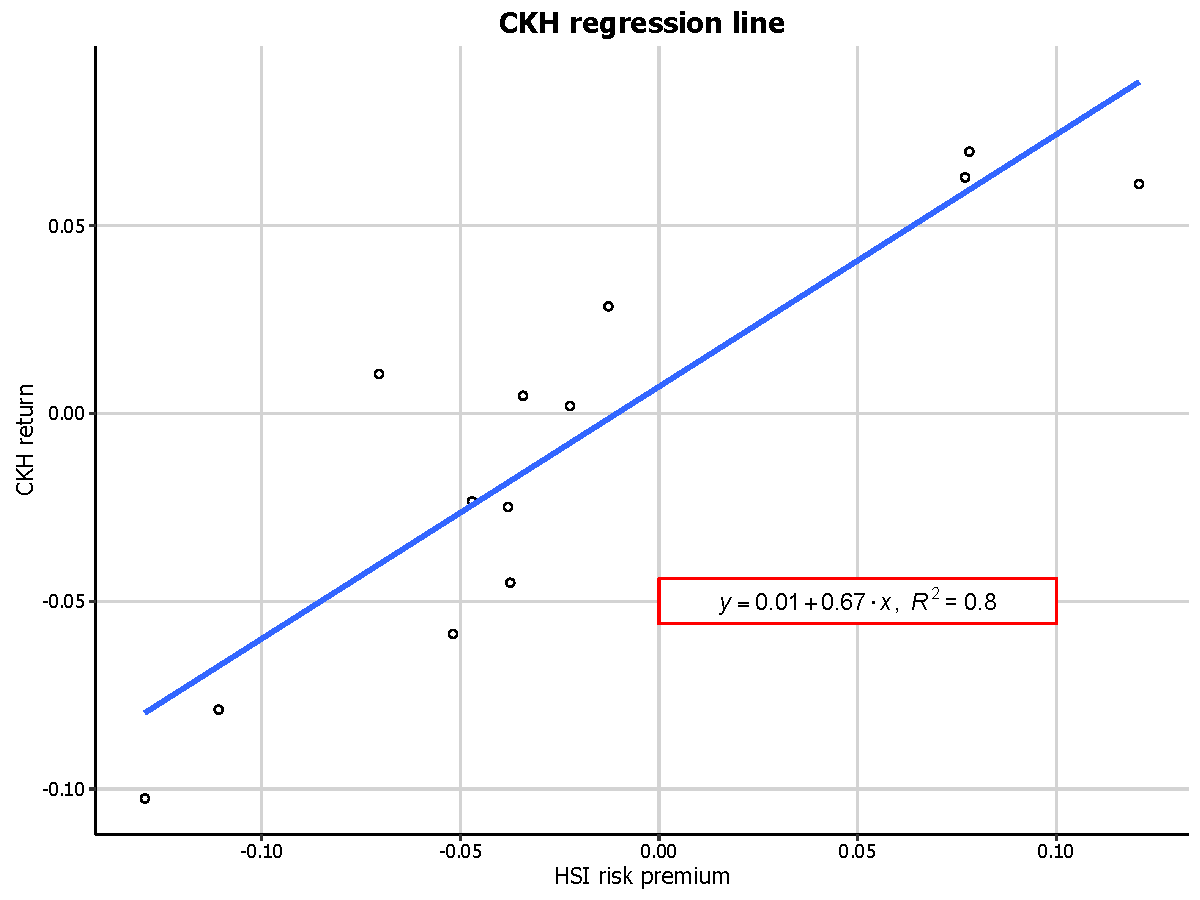
\includegraphics[width=0.55\linewidth]{figures/lr_final-1} \end{center}

\begin{center}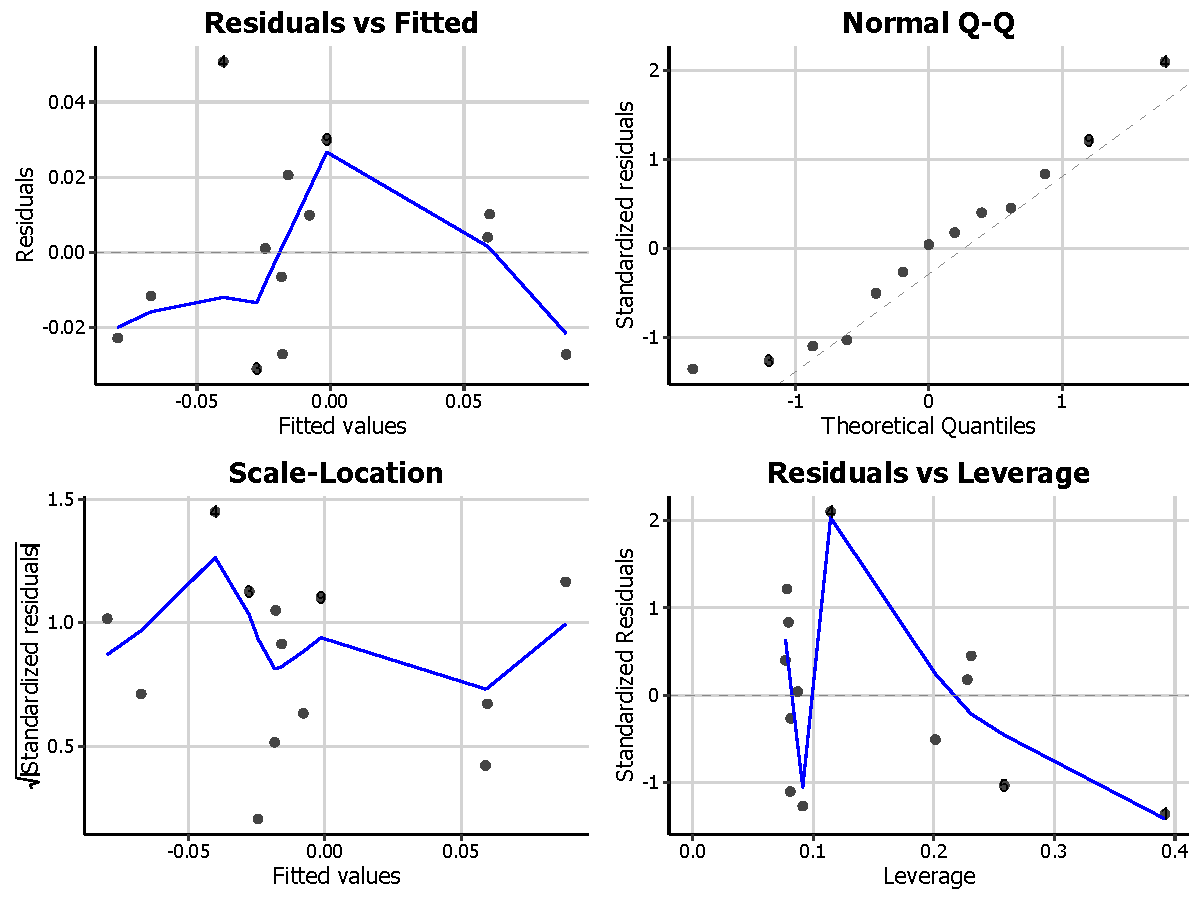
\includegraphics[width=0.55\linewidth]{figures/lr_final-2} \end{center}

The first thing to do is download and load in the data of the monthly
price of Hang Seng Index and Cheung Kong Holdings Hong Kong from
2015-03-01 to 2016-04-01.

\begin{Shaded}
\begin{Highlighting}[]
\KeywordTok{library}\NormalTok{(ggplot2)}
\KeywordTok{library}\NormalTok{(Quandl)}
\NormalTok{Quandl.api_key("XXX")}

\NormalTok{hsi.df <-}\StringTok{ }\KeywordTok{Quandl}\NormalTok{(}\StringTok{"YAHOO/INDEX_HSI"}\NormalTok{, }\DataTypeTok{start_date=}\StringTok{"2015-03-01"}\NormalTok{, }
\StringTok{           }\DataTypeTok{end_date=}\StringTok{"2016-04-01"}\NormalTok{,}\DataTypeTok{collapse=}\StringTok{"monthly"}\NormalTok{, }\DataTypeTok{type =} \StringTok{"raw"}\NormalTok{, }
\StringTok{           }\NormalTok{)}

\NormalTok{ckh.df <-}\StringTok{ }\KeywordTok{Quandl}\NormalTok{(}\StringTok{"YAHOO/HK_0001"}\NormalTok{, }\DataTypeTok{start_date=}\StringTok{"2015-03-01"}\NormalTok{, }
\StringTok{           }\DataTypeTok{end_date=}\StringTok{"2016-04-01"}\NormalTok{, }\DataTypeTok{collapse=}\StringTok{"monthly"}\NormalTok{, }\DataTypeTok{type =} \StringTok{"raw"}\NormalTok{, }
\StringTok{           }\NormalTok{)}

\KeywordTok{saveRDS}\NormalTok{(hsi.df, }\StringTok{"hsi.rds"}\NormalTok{); }\KeywordTok{saveRDS}\NormalTok{(ckh.df,}\StringTok{"ckh.rds"}\NormalTok{)}
\end{Highlighting}
\end{Shaded}

Before calculating return as
\(R_i = \displaystyle \frac{P_t - P_{t-1}}{P_t}\) it is needed to order
HSI and CKH data by dates and in decreasing order.

\begin{Shaded}
\begin{Highlighting}[]
\NormalTok{hsi.df <-}\StringTok{ }\KeywordTok{readRDS}\NormalTok{(}\StringTok{"hsi.rds"}\NormalTok{)}
\KeywordTok{colnames}\NormalTok{(hsi.df)[}\DecValTok{7}\NormalTok{] <-}\StringTok{ "Adjusted.Close"}
\NormalTok{hsi.df <-}\StringTok{ }\NormalTok{hsi.df[}\KeywordTok{order}\NormalTok{(}\KeywordTok{as.Date}\NormalTok{(hsi.df$Date)),]}
\end{Highlighting}
\end{Shaded}

With ordered dates it is possible to obtain the correct return for each
month.

\begin{Shaded}
\begin{Highlighting}[]
\NormalTok{hsi.Adjusted.Close <-}\StringTok{ }\NormalTok{hsi.df$Adjusted.Close}
\NormalTok{hsi.Return <-}\StringTok{ }\KeywordTok{diff}\NormalTok{(hsi.Adjusted.Close)/}
\StringTok{        }\NormalTok{hsi.Adjusted.Close[-}\KeywordTok{length}\NormalTok{(hsi.Adjusted.Close)]}
\NormalTok{hsi.Return <-}\StringTok{ }\KeywordTok{c}\NormalTok{(}\OtherTok{NA}\NormalTok{,hsi.Return)}
\NormalTok{hsi.df$Return <-}\StringTok{ }\NormalTok{hsi.Return}
\NormalTok{hsi.df <-}\StringTok{ }\KeywordTok{na.omit}\NormalTok{(hsi.df)}
\NormalTok{hsi.Return <-}\StringTok{ }\NormalTok{hsi.df[,}\KeywordTok{c}\NormalTok{(}\StringTok{"Date"}\NormalTok{,}\StringTok{"Return"}\NormalTok{)]}

\NormalTok{ckh.df <-}\StringTok{ }\KeywordTok{readRDS}\NormalTok{(}\StringTok{"ckh.rds"}\NormalTok{)}
\KeywordTok{colnames}\NormalTok{(ckh.df)[}\DecValTok{7}\NormalTok{] <-}\StringTok{ "Adjusted.Close"}
\NormalTok{ckh.df <-}\StringTok{ }\NormalTok{ckh.df[}\KeywordTok{order}\NormalTok{(}\KeywordTok{as.Date}\NormalTok{(ckh.df$Date)),]}
\NormalTok{ckh.Adjusted.Close <-}\StringTok{ }\NormalTok{ckh.df$Adjusted.Close}
\NormalTok{ckh.Return <-}\StringTok{ }\KeywordTok{diff}\NormalTok{(ckh.Adjusted.Close)/}
\StringTok{        }\NormalTok{ckh.Adjusted.Close[-}\KeywordTok{length}\NormalTok{(ckh.Adjusted.Close)]}
\NormalTok{ckh.Return <-}\StringTok{ }\KeywordTok{c}\NormalTok{(}\OtherTok{NA}\NormalTok{,ckh.Return)}
\NormalTok{ckh.df <-}\StringTok{ }\KeywordTok{na.omit}\NormalTok{(ckh.df)}
\NormalTok{ckh.df$Return <-}\StringTok{ }\NormalTok{ckh.Return}
\NormalTok{ckh.Return <-}\StringTok{ }\NormalTok{ckh.df[,}\KeywordTok{c}\NormalTok{(}\StringTok{"Date"}\NormalTok{,}\StringTok{"Return"}\NormalTok{)]}
\end{Highlighting}
\end{Shaded}

The returns can be arranged in one data frame before doing plots and
regression.

\begin{Shaded}
\begin{Highlighting}[]
\NormalTok{hsi.ckh.returns <-}\StringTok{ }\KeywordTok{merge}\NormalTok{(hsi.Return, ckh.Return, }\DataTypeTok{by=}\StringTok{'Date'}\NormalTok{)}
\NormalTok{hsi.ckh.returns <-}\StringTok{ }\KeywordTok{na.omit}\NormalTok{(hsi.ckh.returns)}
\KeywordTok{colnames}\NormalTok{(hsi.ckh.returns) <-}\StringTok{ }\KeywordTok{c}\NormalTok{(}\StringTok{"Date"}\NormalTok{,}\StringTok{"hsi.Return"}\NormalTok{,}\StringTok{"ckh.Return"}\NormalTok{)}
\end{Highlighting}
\end{Shaded}

Using
\href{http://pages.stern.nyu.edu/~adamodar/New_Home_Page/datafile/ctryprem.html}{Damodaran}
and
\href{http://www.bloomberg.com/markets/rates-bonds/government-bonds/us}{Bloomberg}
data we can work with an estimate of HSI risk premium over risk-free
rate.

\begin{Shaded}
\begin{Highlighting}[]
\NormalTok{usa.risk.free <-}\StringTok{ }\FloatTok{0.3}\NormalTok{/}\DecValTok{100}
\NormalTok{hsi.risk.premium <-}\StringTok{ }\FloatTok{0.6}\NormalTok{/}\DecValTok{100}
\end{Highlighting}
\end{Shaded}

\section{Trend line plot}\label{trend-line-plot}

\subsection{Basic trend line plot}\label{basic-trend-line-plot}

Now we can fit a linear regression. %One interesting thing is that in
%CAPM context the regression line slope can be calculated as
%\(\beta_i = \displaystyle \frac{\sigma_{i,m}}{\sigma_m^2}\).

\begin{Shaded}
\begin{Highlighting}[]
\NormalTok{fit <-}\StringTok{ }\KeywordTok{lm}\NormalTok{(ckh.Return ~}\StringTok{ }\NormalTok{hsi.Risk.premium, }\DataTypeTok{data =} \NormalTok{hsi.ckh.returns) }
\KeywordTok{summary}\NormalTok{(fit)}
\end{Highlighting}
\end{Shaded}

\begin{verbatim}

Call:
lm(formula = ckh.Return ~ hsi.Risk.premium, data = hsi.ckh.returns)

Residuals:
      Min        1Q    Median        3Q       Max 
-0.031033 -0.022800  0.001032  0.010137  0.050709 

Coefficients:
\StringTok{       }Estimate Std. Error t value Pr(>|t|)    
(Intercept)      0.007142   0.007437   0.960    0.357    
hsi.Risk.premium 0.671372   0.101209   6.634 3.69e-05 ***
---
Signif. codes:  0 '***' 0.001 '**' 0.01 '*' 0.05 '.' 0.1 ' ' 1

Residual standard error: 0.02565 on 11 degrees of freedom
Multiple R-squared:    0.8, Adjusted R-squared:  0.7818 
F-statistic:    44 on 1 and 11 DF,  p-value: 3.692e-05
\end{verbatim}

Up to this point we have all what is required to plot regressions. We
will start with a basic regression plot.

\begin{Shaded}
\begin{Highlighting}[]
\NormalTok{p11 <-}\StringTok{ }\KeywordTok{ggplot}\NormalTok{(hsi.ckh.returns, }\KeywordTok{aes}\NormalTok{(}\DataTypeTok{x=}\NormalTok{hsi.Risk.premium, }\DataTypeTok{y=}\NormalTok{ckh.Return)) +}
\StringTok{      }\StringTok{ }\KeywordTok{geom_point}\NormalTok{(}\DataTypeTok{shape=}\DecValTok{1}\NormalTok{) +}\StringTok{ }\KeywordTok{geom_smooth}\NormalTok{(}\DataTypeTok{method=}\NormalTok{lm) }
\NormalTok{p11}
\end{Highlighting}
\end{Shaded}

\begin{center}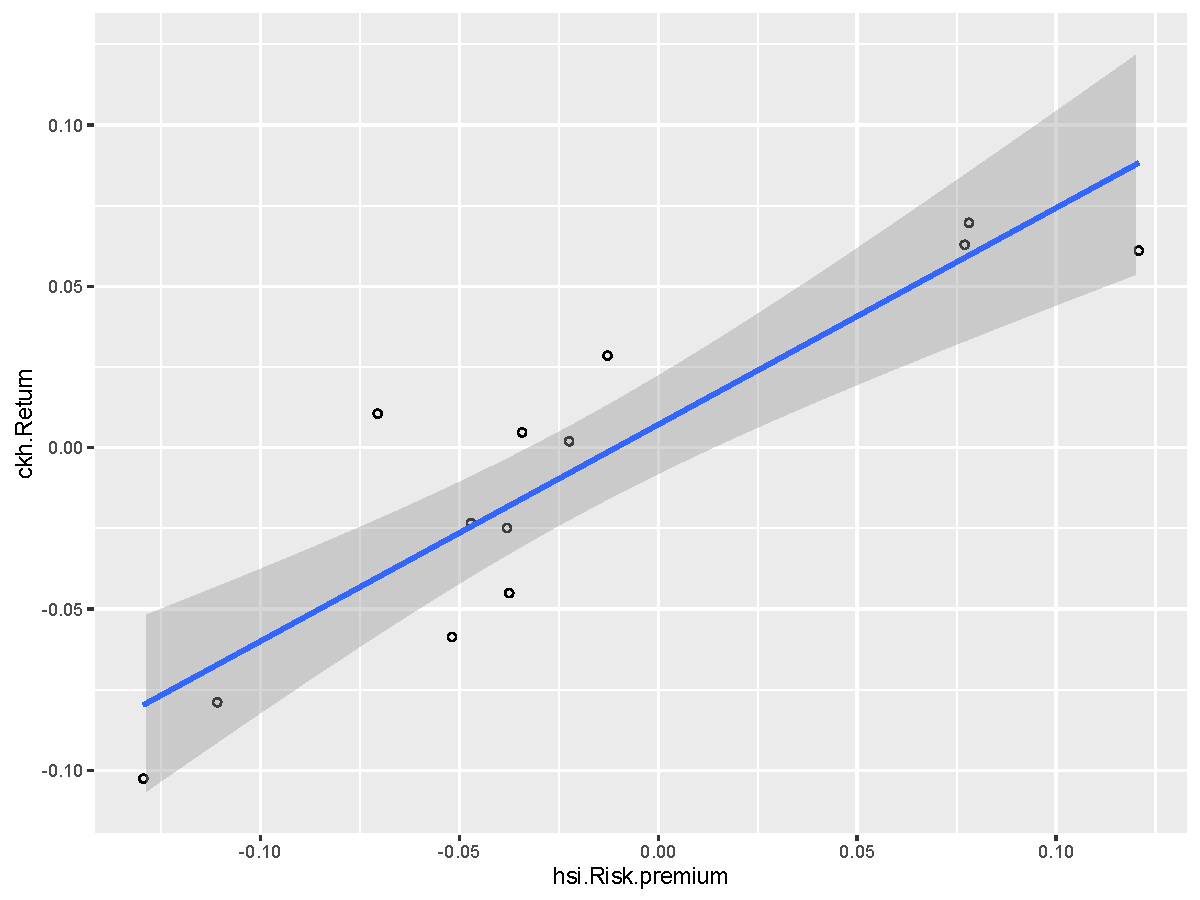
\includegraphics[width=0.55\linewidth]{figures/lr_6-1} \end{center}

\texttt{geom\_point} can be customized, for example, not to include the
confidence region

\begin{Shaded}
\begin{Highlighting}[]
\NormalTok{p11 <-}\StringTok{ }\KeywordTok{ggplot}\NormalTok{(hsi.ckh.returns, }\KeywordTok{aes}\NormalTok{(}\DataTypeTok{x=}\NormalTok{hsi.Risk.premium, }\DataTypeTok{y=}\NormalTok{ckh.Return)) +}
\StringTok{       }\KeywordTok{geom_point}\NormalTok{(}\DataTypeTok{shape=}\DecValTok{1}\NormalTok{) +}\StringTok{ }\KeywordTok{geom_smooth}\NormalTok{(}\DataTypeTok{method=}\NormalTok{lm, }\DataTypeTok{se=}\OtherTok{FALSE}\NormalTok{) }
\NormalTok{p11}
\end{Highlighting}
\end{Shaded}

\begin{center}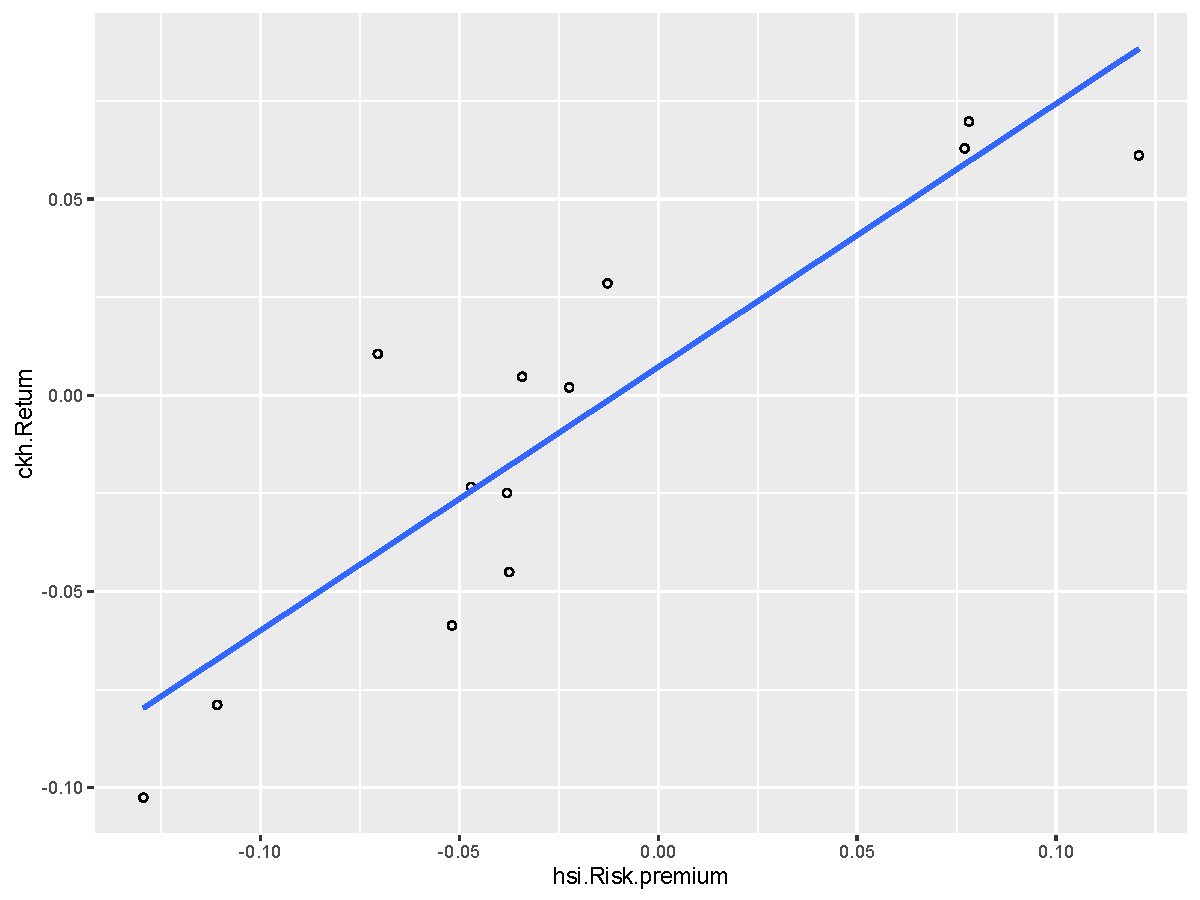
\includegraphics[width=0.55\linewidth]{figures/lr_7-1} \end{center}

Before continuing it is a good idea to fix the axis labels and add a
title.

\subsection{Customising axis labels}\label{customising-axis-labels-4}

\begin{Shaded}
\begin{Highlighting}[]
\NormalTok{p11 <-}\StringTok{ }\NormalTok{p11 +}\StringTok{ }\KeywordTok{scale_x_continuous}\NormalTok{(}\DataTypeTok{name =} \StringTok{"HSI risk premium"}\NormalTok{) +}\StringTok{ }
\StringTok{       }\KeywordTok{scale_y_continuous}\NormalTok{(}\DataTypeTok{name =} \StringTok{"CKH return"}\NormalTok{)}
\NormalTok{p11}
\end{Highlighting}
\end{Shaded}

\begin{center}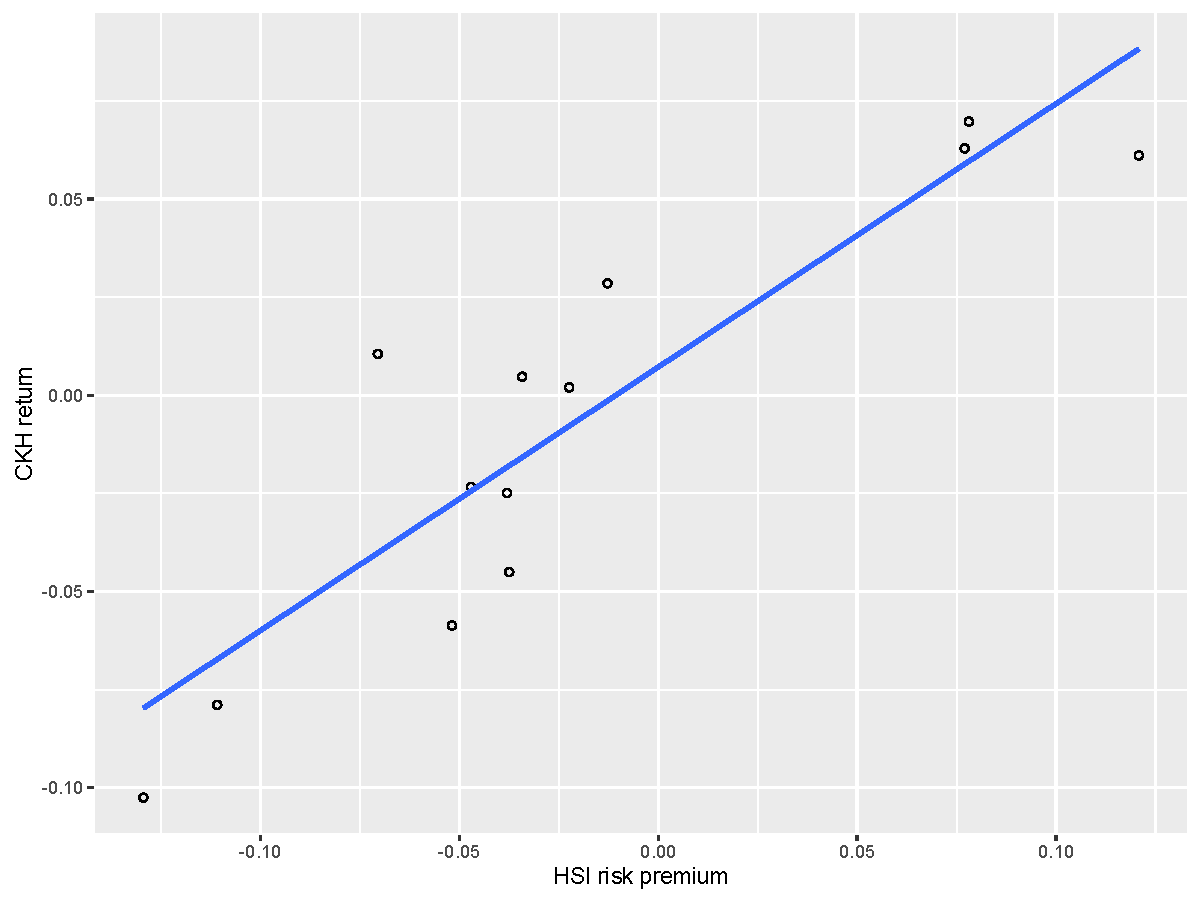
\includegraphics[width=0.55\linewidth]{figures/lr_8-1} \end{center}

\subsection{Adding a title}\label{adding-a-title-4}

\begin{Shaded}
\begin{Highlighting}[]
\NormalTok{p11 <-}\StringTok{ }\NormalTok{p11 +}\StringTok{ }\KeywordTok{ggtitle}\NormalTok{(}\StringTok{"CKH regression line"}\NormalTok{)}
\NormalTok{p11}
\end{Highlighting}
\end{Shaded}

\begin{center}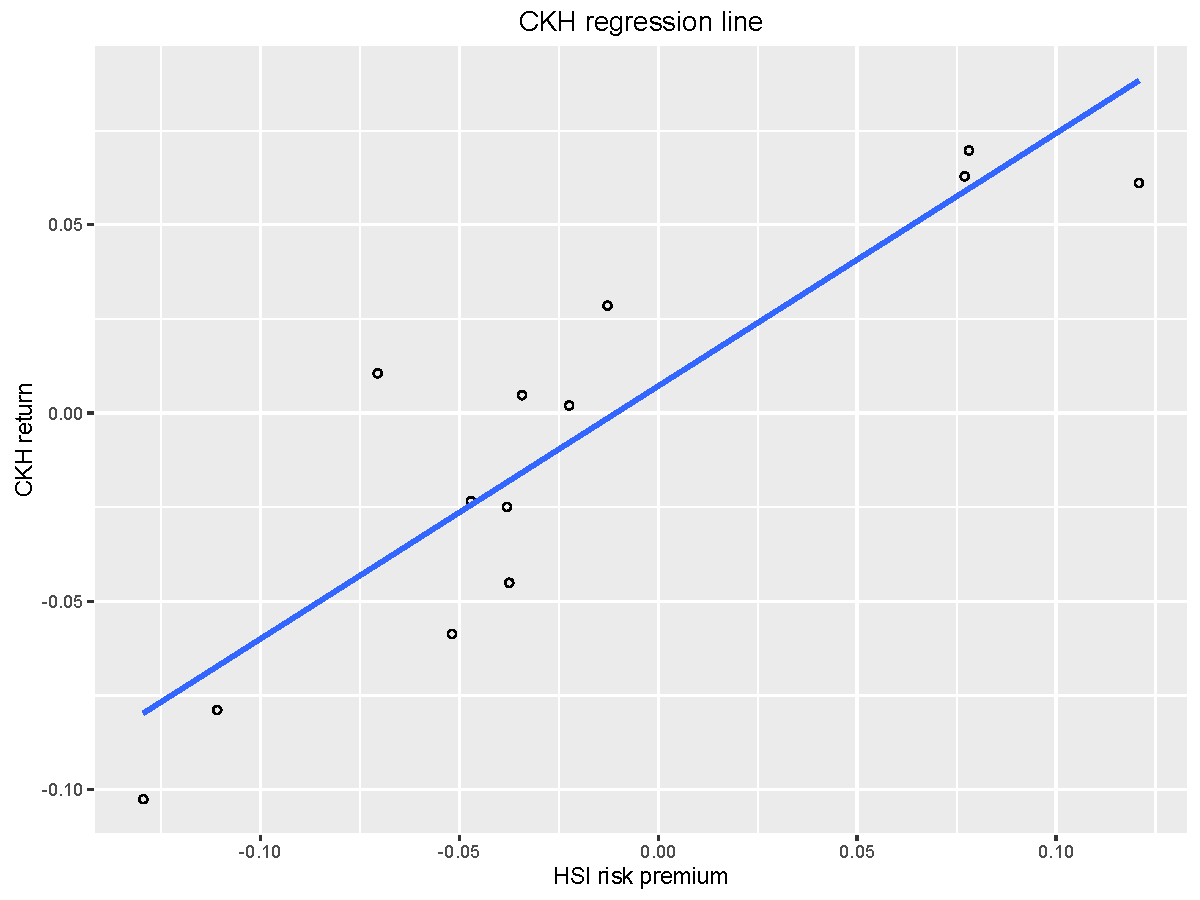
\includegraphics[width=0.55\linewidth]{figures/lr_9-1} \end{center}

\subsection{Including regression
coefficients}\label{including-regression-coefficients}

It would be interesting to show \(R^2\) and regression coefficients
within the plot.

\begin{Shaded}
\begin{Highlighting}[]
\NormalTok{p11 <-}\StringTok{ }\NormalTok{p11 +}\StringTok{ }\KeywordTok{annotate}\NormalTok{(}\StringTok{"text"}\NormalTok{, }\DataTypeTok{x=}\FloatTok{0.1}\NormalTok{, }\DataTypeTok{y=}\NormalTok{-}\FloatTok{0.05}\NormalTok{, }\DataTypeTok{label =} \StringTok{"R^2=0.78"}\NormalTok{) +}\StringTok{ }
\StringTok{       }\KeywordTok{annotate}\NormalTok{(}\StringTok{"text"}\NormalTok{, }\DataTypeTok{x=}\FloatTok{0.1}\NormalTok{, }\DataTypeTok{y=}\NormalTok{-}\FloatTok{0.06}\NormalTok{, }\DataTypeTok{label =} \StringTok{"alpha=0.00"}\NormalTok{) +}\StringTok{ }
\StringTok{       }\KeywordTok{annotate}\NormalTok{(}\StringTok{"text"}\NormalTok{, }\DataTypeTok{x=}\FloatTok{0.1}\NormalTok{, }\DataTypeTok{y=}\NormalTok{-}\FloatTok{0.07}\NormalTok{, }\DataTypeTok{label =} \StringTok{"beta=0.67"}\NormalTok{)}
\NormalTok{p11}
\end{Highlighting}
\end{Shaded}

\begin{center}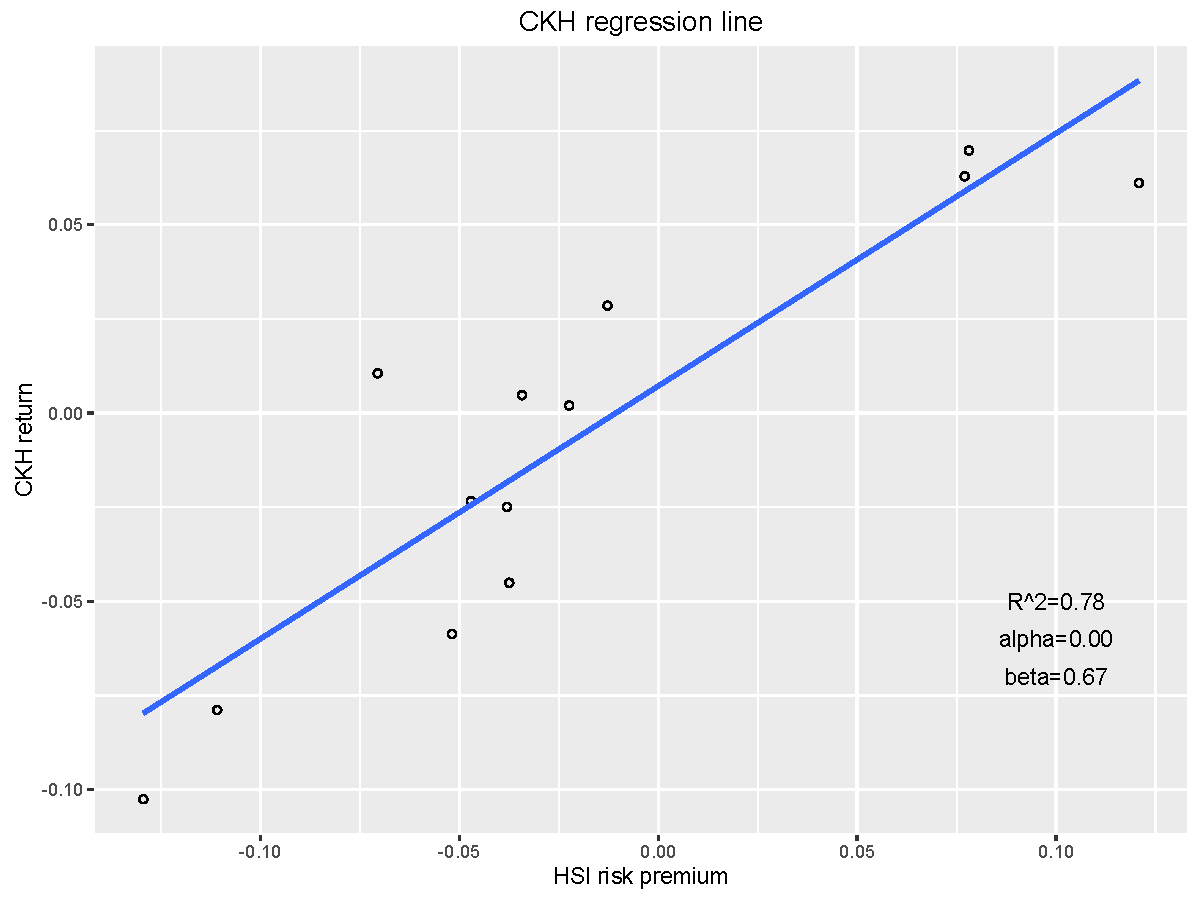
\includegraphics[width=0.55\linewidth]{figures/lr_10-1} \end{center}

Another option would be to add greek letters and exponents.

\begin{Shaded}
\begin{Highlighting}[]
\NormalTok{p11 <-}\StringTok{ }\KeywordTok{ggplot}\NormalTok{(hsi.ckh.returns, }\KeywordTok{aes}\NormalTok{(}\DataTypeTok{x=}\NormalTok{hsi.Risk.premium, }\DataTypeTok{y=}\NormalTok{ckh.Return)) +}
\StringTok{       }\KeywordTok{geom_point}\NormalTok{(}\DataTypeTok{shape=}\DecValTok{1}\NormalTok{) +}\StringTok{ }
\StringTok{       }\KeywordTok{geom_smooth}\NormalTok{(}\DataTypeTok{method=}\NormalTok{lm, }\DataTypeTok{se=}\OtherTok{FALSE}\NormalTok{) +}\StringTok{ }\KeywordTok{ggtitle}\NormalTok{(}\StringTok{"CKH regression line"}\NormalTok{) +}
\StringTok{       }\KeywordTok{scale_x_continuous}\NormalTok{(}\DataTypeTok{name =} \StringTok{"HSI risk premium"}\NormalTok{) +}
\StringTok{       }\KeywordTok{scale_y_continuous}\NormalTok{(}\DataTypeTok{name =} \StringTok{"CKH return"}\NormalTok{) +}\StringTok{ }
\StringTok{       }\KeywordTok{annotate}\NormalTok{(}\StringTok{"text"}\NormalTok{, }\DataTypeTok{x=}\FloatTok{0.1}\NormalTok{, }\DataTypeTok{y=}\NormalTok{-}\FloatTok{0.05}\NormalTok{, }\DataTypeTok{label =} \StringTok{"R^2 == 0.78"}\NormalTok{, }\DataTypeTok{parse=}\NormalTok{T) +}\StringTok{ }
\StringTok{       }\KeywordTok{annotate}\NormalTok{(}\StringTok{"text"}\NormalTok{, }\DataTypeTok{x=}\FloatTok{0.1}\NormalTok{, }\DataTypeTok{y=}\NormalTok{-}\FloatTok{0.06}\NormalTok{, }\DataTypeTok{label =} \StringTok{"alpha == 0.00"}\NormalTok{, }\DataTypeTok{parse=}\NormalTok{T) +}\StringTok{ }
\StringTok{       }\KeywordTok{annotate}\NormalTok{(}\StringTok{"text"}\NormalTok{, }\DataTypeTok{x=}\FloatTok{0.1}\NormalTok{, }\DataTypeTok{y=}\NormalTok{-}\FloatTok{0.07}\NormalTok{, }\DataTypeTok{label =} \StringTok{"beta == 0.67"}\NormalTok{, }\DataTypeTok{parse=}\NormalTok{T)}
\NormalTok{p11}
\end{Highlighting}
\end{Shaded}

\begin{center}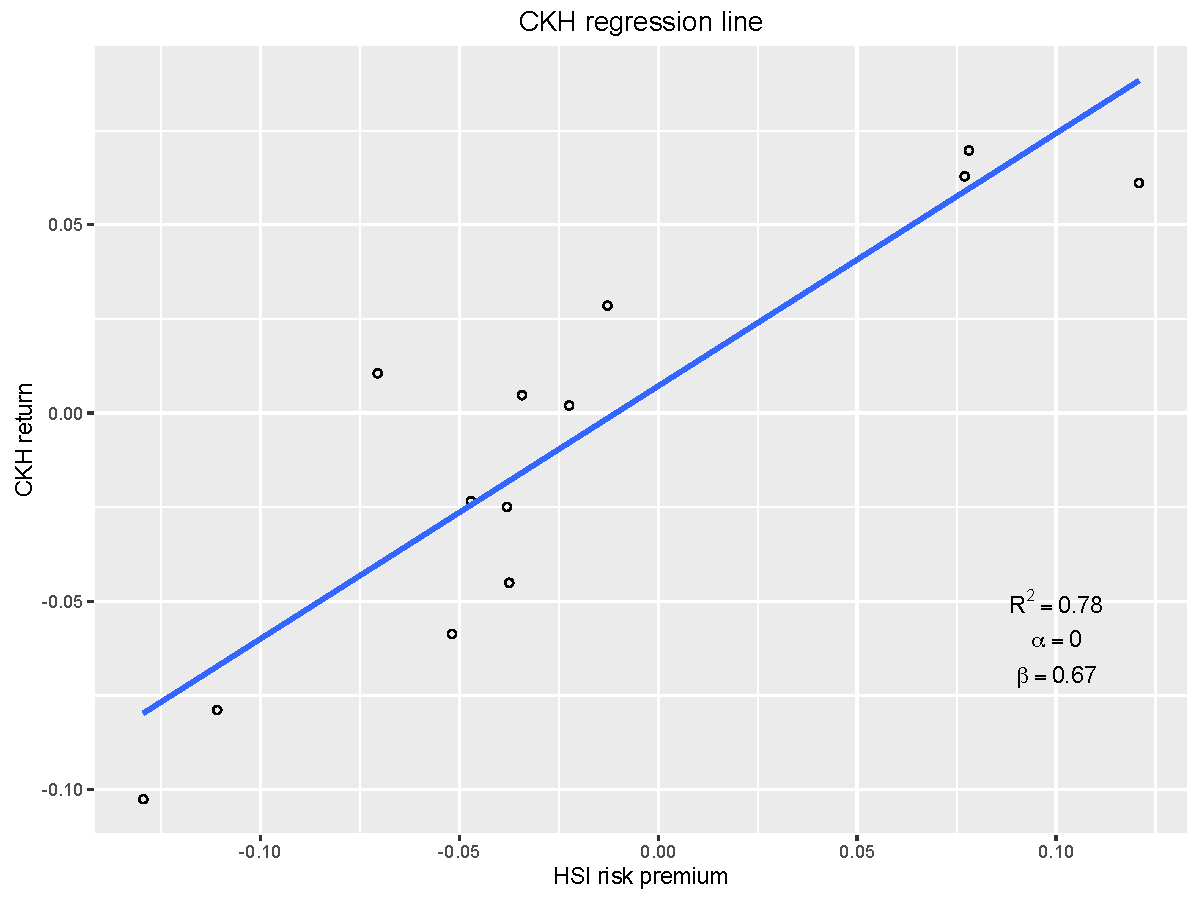
\includegraphics[width=0.55\linewidth]{figures/lr_11-1} \end{center}

To make the coefficients more visible we will add some elements to
increase visibility

\begin{Shaded}
\begin{Highlighting}[]
\NormalTok{p11 <-}\StringTok{ }\KeywordTok{ggplot}\NormalTok{(hsi.ckh.returns, }\KeywordTok{aes}\NormalTok{(}\DataTypeTok{x=}\NormalTok{hsi.Risk.premium, }\DataTypeTok{y=}\NormalTok{ckh.Return)) +}\StringTok{ }
\StringTok{       }\KeywordTok{geom_point}\NormalTok{(}\DataTypeTok{shape=}\DecValTok{1}\NormalTok{) +}\StringTok{ }\KeywordTok{geom_smooth}\NormalTok{(}\DataTypeTok{method=}\NormalTok{lm, }\DataTypeTok{se=}\OtherTok{FALSE}\NormalTok{) +}
\StringTok{       }\KeywordTok{ggtitle}\NormalTok{(}\StringTok{"CKH regression line"}\NormalTok{) +}
\StringTok{       }\KeywordTok{scale_x_continuous}\NormalTok{(}\DataTypeTok{name =} \StringTok{"HSI risk premium"}\NormalTok{) +}
\StringTok{       }\KeywordTok{scale_y_continuous}\NormalTok{(}\DataTypeTok{name =} \StringTok{"CKH return"}\NormalTok{) +}
\StringTok{       }\KeywordTok{annotate}\NormalTok{(}\StringTok{"rect"}\NormalTok{, }\DataTypeTok{xmin =} \FloatTok{0.075}\NormalTok{, }\DataTypeTok{xmax =} \FloatTok{0.125}\NormalTok{, }\DataTypeTok{ymin =} \NormalTok{-}\FloatTok{0.075}\NormalTok{, }
\StringTok{        }\DataTypeTok{ymax =} \NormalTok{-}\FloatTok{0.045}\NormalTok{, }\DataTypeTok{fill=}\StringTok{"white"}\NormalTok{, }\DataTypeTok{colour=}\StringTok{"red"}\NormalTok{) +}\StringTok{ }
\StringTok{       }\KeywordTok{annotate}\NormalTok{(}\StringTok{"text"}\NormalTok{, }\DataTypeTok{x=}\FloatTok{0.1}\NormalTok{, }\DataTypeTok{y=}\NormalTok{-}\FloatTok{0.05}\NormalTok{, }\DataTypeTok{label =} \StringTok{"R^2 == 0.78"}\NormalTok{, }\DataTypeTok{parse=}\NormalTok{T) +}
\StringTok{       }\KeywordTok{annotate}\NormalTok{(}\StringTok{"text"}\NormalTok{, }\DataTypeTok{x=}\FloatTok{0.1}\NormalTok{, }\DataTypeTok{y=}\NormalTok{-}\FloatTok{0.06}\NormalTok{, }\DataTypeTok{label =} \StringTok{"alpha == 0.00"}\NormalTok{, }\DataTypeTok{parse=}\NormalTok{T) +}\StringTok{ }
\StringTok{       }\KeywordTok{annotate}\NormalTok{(}\StringTok{"text"}\NormalTok{, }\DataTypeTok{x=}\FloatTok{0.1}\NormalTok{, }\DataTypeTok{y=}\NormalTok{-}\FloatTok{0.07}\NormalTok{, }\DataTypeTok{label =} \StringTok{"beta == 0.67"}\NormalTok{, }\DataTypeTok{parse=}\NormalTok{T)}
\NormalTok{p11}
\end{Highlighting}
\end{Shaded}

\begin{center}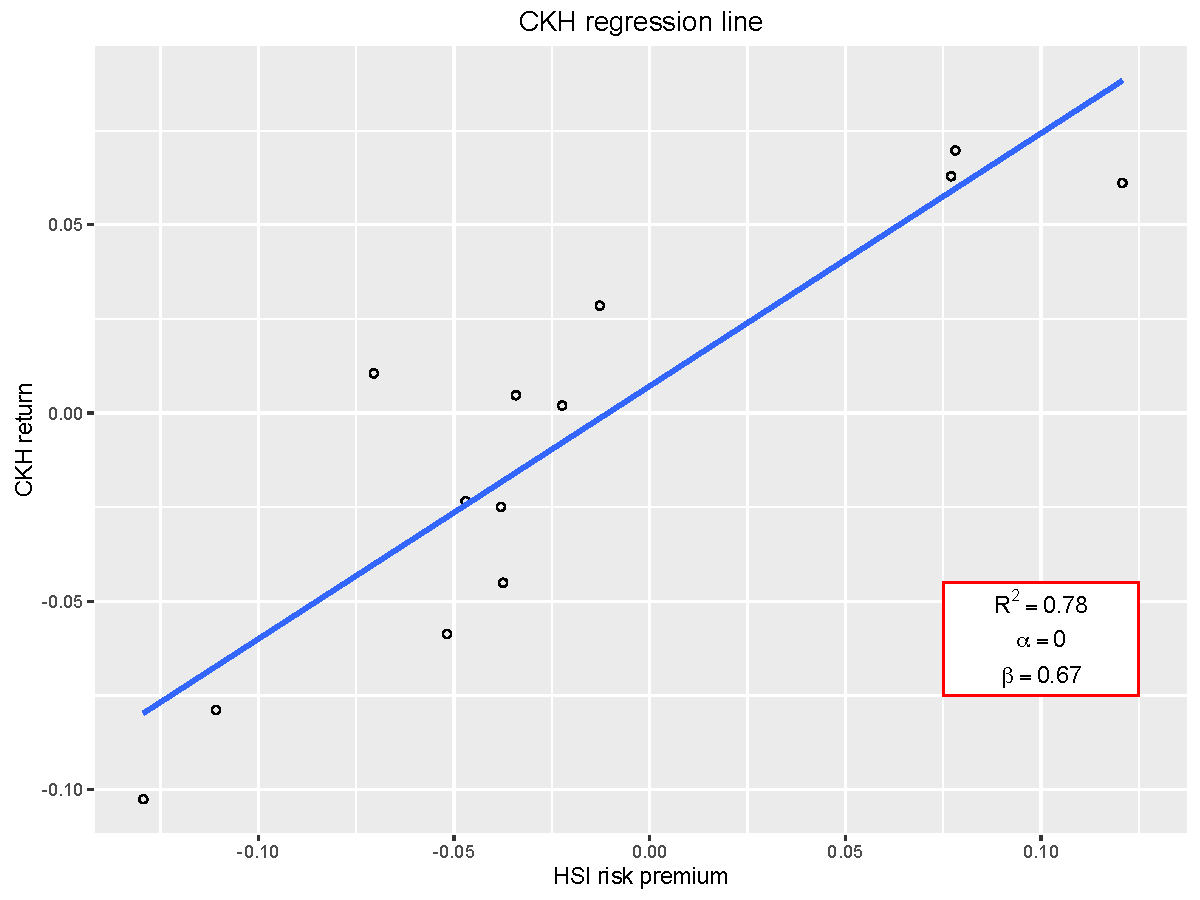
\includegraphics[width=0.55\linewidth]{figures/lr_12-1} \end{center}

Another customization could be to show the trend line using rounded
digits (or even significative digits) from regression coefficients. This
requires us to write a function and is not as easy to obtain as the last
plot.

\begin{Shaded}
\begin{Highlighting}[]
\NormalTok{equation =}\StringTok{ }\NormalTok{function(x) \{}
  \NormalTok{lm_coef <-}\StringTok{ }\KeywordTok{list}\NormalTok{(}\DataTypeTok{a =} \KeywordTok{round}\NormalTok{(}\KeywordTok{coef}\NormalTok{(x)[}\DecValTok{1}\NormalTok{], }\DataTypeTok{digits =} \DecValTok{2}\NormalTok{),}
\StringTok{       }\DataTypeTok{b =} \KeywordTok{round}\NormalTok{(}\KeywordTok{coef}\NormalTok{(x)[}\DecValTok{2}\NormalTok{], }\DataTypeTok{digits =} \DecValTok{2}\NormalTok{),}
\StringTok{       }\DataTypeTok{r2 =} \KeywordTok{round}\NormalTok{(}\KeywordTok{summary}\NormalTok{(x)$r.squared, }\DataTypeTok{digits =} \DecValTok{2}\NormalTok{));}
  \NormalTok{lm_eq <-}\StringTok{ }\KeywordTok{substitute}\NormalTok{(}\KeywordTok{italic}\NormalTok{(y) ==}\StringTok{ }\NormalTok{a +}\StringTok{ }\NormalTok{b %.%}\StringTok{ }\KeywordTok{italic}\NormalTok{(x)*}\StringTok{","}\NormalTok{~}\ErrorTok{~}\KeywordTok{italic}\NormalTok{(R)^}\DecValTok{2}\NormalTok{~}\StringTok{"="}~r2,
\StringTok{       }lm_coef)
  \KeywordTok{as.character}\NormalTok{(}\KeywordTok{as.expression}\NormalTok{(lm_eq));\StringTok{       }}
\NormalTok{\}}

\NormalTok{p11 <-}\StringTok{ }\KeywordTok{ggplot}\NormalTok{(hsi.ckh.returns, }\KeywordTok{aes}\NormalTok{(}\DataTypeTok{x=}\NormalTok{hsi.Risk.premium, }\DataTypeTok{y=}\NormalTok{ckh.Return)) +}
\StringTok{       }\KeywordTok{geom_point}\NormalTok{(}\DataTypeTok{shape=}\DecValTok{1}\NormalTok{) +}\StringTok{ }\KeywordTok{geom_smooth}\NormalTok{(}\DataTypeTok{method=}\NormalTok{lm, }\DataTypeTok{se=}\OtherTok{FALSE}\NormalTok{) +}
\StringTok{       }\KeywordTok{ggtitle}\NormalTok{(}\StringTok{"CKH regression line"}\NormalTok{) +}
\StringTok{       }\KeywordTok{scale_x_continuous}\NormalTok{(}\DataTypeTok{name =} \StringTok{"HSI risk premium"}\NormalTok{) +}
\StringTok{       }\KeywordTok{scale_y_continuous}\NormalTok{(}\DataTypeTok{name =} \StringTok{"CKH return"}\NormalTok{) +}
\StringTok{       }\KeywordTok{annotate}\NormalTok{(}\StringTok{"rect"}\NormalTok{, }\DataTypeTok{xmin =} \FloatTok{0.00}\NormalTok{, }\DataTypeTok{xmax =} \FloatTok{0.1}\NormalTok{, }\DataTypeTok{ymin =} \NormalTok{-}\FloatTok{0.056}\NormalTok{, }\DataTypeTok{ymax =} \NormalTok{-}\FloatTok{0.044}\NormalTok{, }
\StringTok{        }\DataTypeTok{fill=}\StringTok{"white"}\NormalTok{, }\DataTypeTok{colour=}\StringTok{"red"}\NormalTok{) +}\StringTok{ }
\StringTok{       }\KeywordTok{annotate}\NormalTok{(}\StringTok{"text"}\NormalTok{, }\DataTypeTok{x =} \FloatTok{0.05}\NormalTok{, }\DataTypeTok{y =} \NormalTok{-}\FloatTok{0.05}\NormalTok{, }\DataTypeTok{label =} \KeywordTok{equation}\NormalTok{(fit), }
\StringTok{        }\DataTypeTok{parse =} \OtherTok{TRUE}\NormalTok{)}
\NormalTok{p11}
\end{Highlighting}
\end{Shaded}

\begin{center}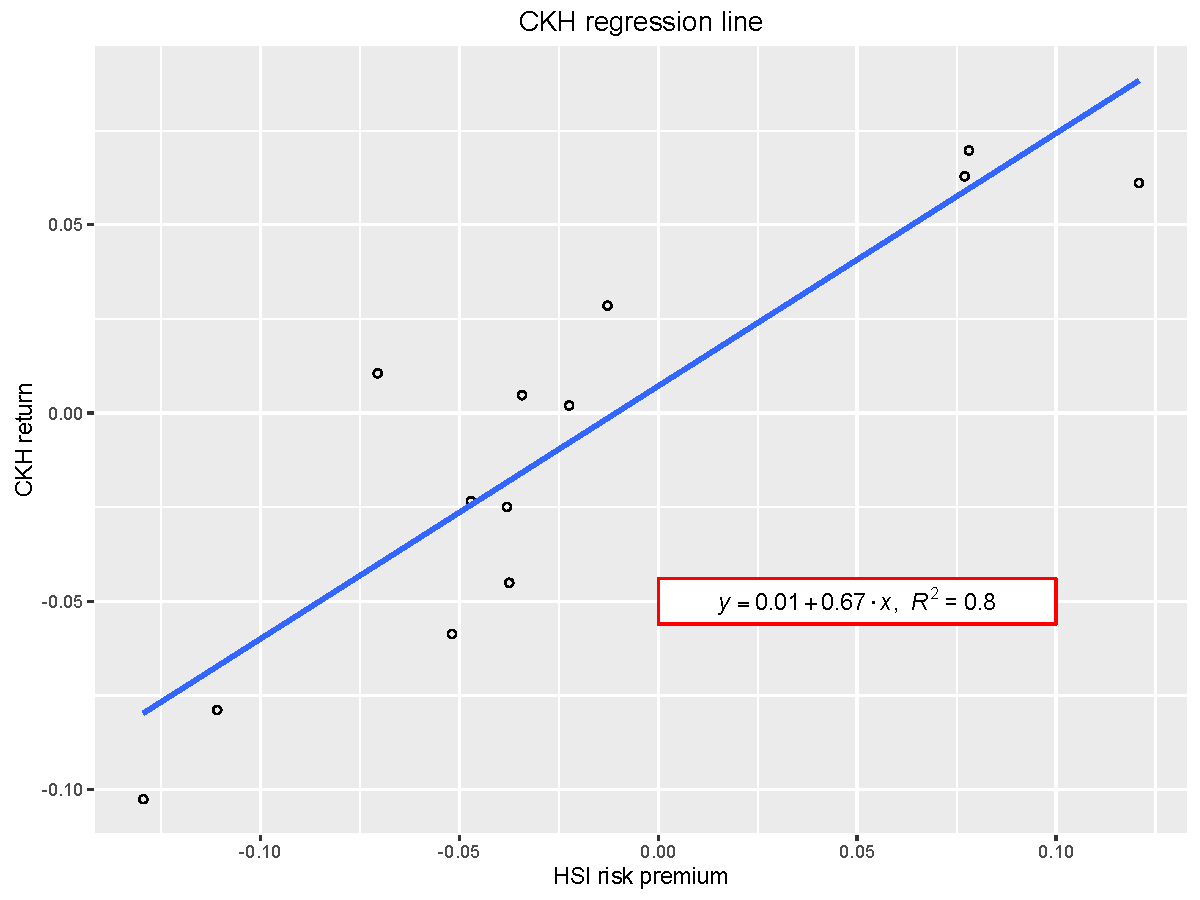
\includegraphics[width=0.55\linewidth]{figures/lr_13-1} \end{center}

\subsection{Using the white theme}\label{using-the-white-theme-10}

\begin{Shaded}
\begin{Highlighting}[]
\NormalTok{p11 <-}\StringTok{ }\NormalTok{p11 +}\StringTok{ }\KeywordTok{theme_bw}\NormalTok{()}
\NormalTok{p11}
\end{Highlighting}
\end{Shaded}

\begin{center}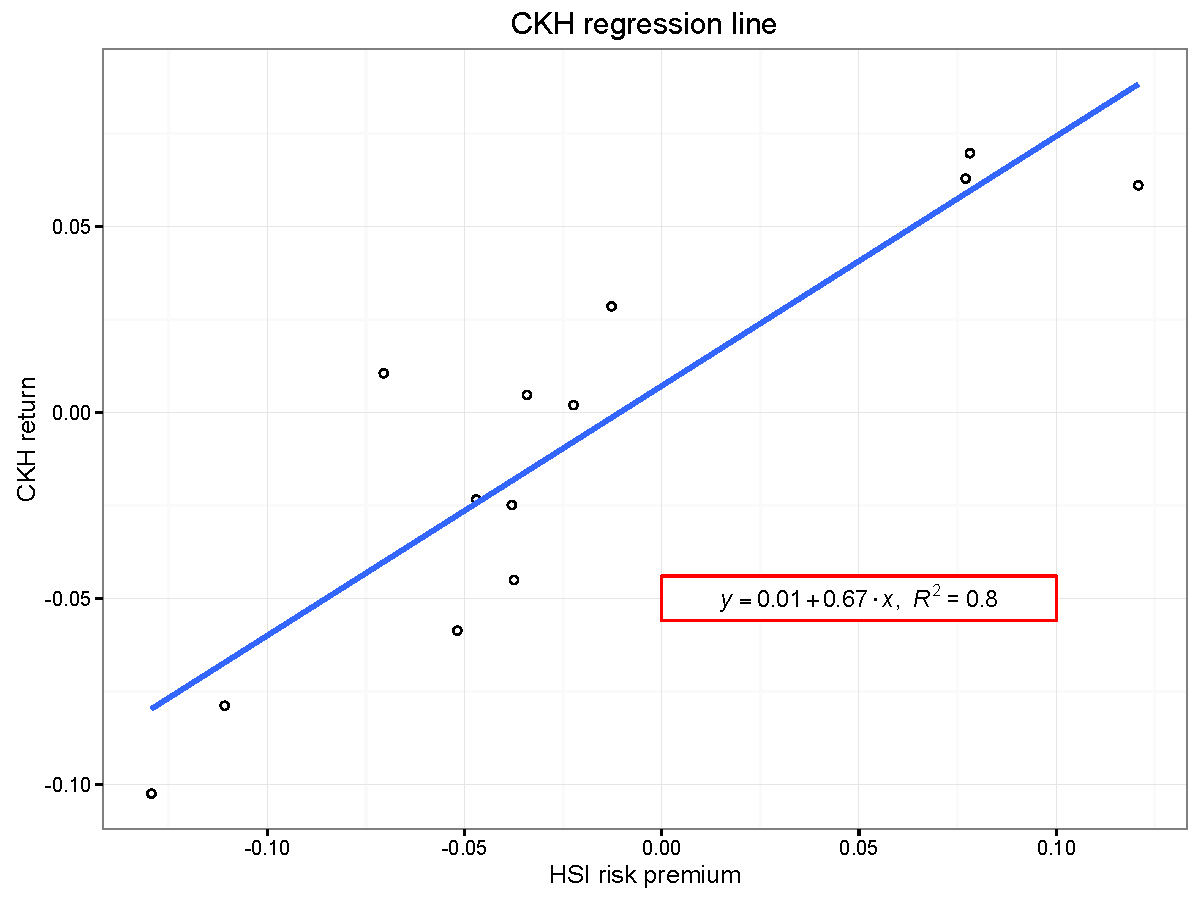
\includegraphics[width=0.55\linewidth]{figures/lr_14-1} \end{center}

\subsection{Creating an XKCD style
chart}\label{creating-an-xkcd-style-chart-10}

Of course, you may want to create your own themes as well.
\texttt{ggplot2} allows for a very high degree of customisation,
including allowing you to use imported fonts. Below is an example of a
theme Mauricio was able to create which mimics the visual style of
\href{http://xkcd.com/}{XKCD}. In order to create this chart, you first
need to import the XKCD font, install it on your machine and load it
into R using the \texttt{extrafont} package. These instructions are
taken from
\href{https://www.google.com.au/url?sa=t\&rct=j\&q=\&esrc=s\&source=web\&cd=1\&ved=0ahUKEwiWzafchdPJAhVBpJQKHe_LDT8QFggbMAA\&url=https\%3A\%2F\%2Fcran.r-project.org\%2Fweb\%2Fpackages\%2Fxkcd\%2Fvignettes\%2Fxkcd-intro.pdf\&usg=AFQjCNE-KciGY14e-Q1buYIVmTFC0ht__Q\&sig2=DZUwkvIHwfNWtTtkcz94jg}{here}:

\begin{Shaded}
\begin{Highlighting}[]
\KeywordTok{library}\NormalTok{(extrafont)}

\KeywordTok{download.file}\NormalTok{(}\StringTok{"http://simonsoftware.se/other/xkcd.ttf"}\NormalTok{, }
\StringTok{       }\DataTypeTok{dest=}\StringTok{"xkcd.ttf"}\NormalTok{, }\DataTypeTok{mode=}\StringTok{"wb"}\NormalTok{)}
\KeywordTok{system}\NormalTok{(}\StringTok{"mkdir ~/.fonts"}\NormalTok{)}
\KeywordTok{system}\NormalTok{(}\StringTok{"cp xkcd.ttf  ~/.fonts"}\NormalTok{)}
\KeywordTok{font_import}\NormalTok{(}\DataTypeTok{paths =} \StringTok{"~/.fonts"}\NormalTok{, }\DataTypeTok{pattern=}\StringTok{"[X/x]kcd"}\NormalTok{)}
\KeywordTok{fonts}\NormalTok{()}
\KeywordTok{loadfonts}\NormalTok{()}
\end{Highlighting}
\end{Shaded}

You can then create your graph:

\begin{Shaded}
\begin{Highlighting}[]
\NormalTok{p11 <-}\StringTok{ }\KeywordTok{ggplot}\NormalTok{(hsi.ckh.returns, }\KeywordTok{aes}\NormalTok{(}\DataTypeTok{x=}\NormalTok{hsi.Risk.premium, }\DataTypeTok{y=}\NormalTok{ckh.Return)) +}
\StringTok{       }\KeywordTok{geom_point}\NormalTok{(}\DataTypeTok{shape=}\DecValTok{1}\NormalTok{) +}\StringTok{ }\KeywordTok{geom_smooth}\NormalTok{(}\DataTypeTok{method=}\NormalTok{lm, }\DataTypeTok{se=}\OtherTok{FALSE}\NormalTok{) +}
\StringTok{       }\KeywordTok{ggtitle}\NormalTok{(}\StringTok{"CKH regression line"}\NormalTok{) +}
\StringTok{       }\KeywordTok{scale_x_continuous}\NormalTok{(}\DataTypeTok{name =} \StringTok{"HSI risk premium"}\NormalTok{) +}
\StringTok{       }\KeywordTok{scale_y_continuous}\NormalTok{(}\DataTypeTok{name =} \StringTok{"CKH return"}\NormalTok{) +}
\StringTok{       }\KeywordTok{annotate}\NormalTok{(}\StringTok{"rect"}\NormalTok{, }\DataTypeTok{xmin =} \FloatTok{0.00}\NormalTok{, }\DataTypeTok{xmax =} \FloatTok{0.1}\NormalTok{, }\DataTypeTok{ymin =} \NormalTok{-}\FloatTok{0.056}\NormalTok{, }\DataTypeTok{ymax =} \NormalTok{-}\FloatTok{0.044}\NormalTok{, }
\StringTok{        }\DataTypeTok{fill=}\StringTok{"white"}\NormalTok{, }\DataTypeTok{colour=}\StringTok{"red"}\NormalTok{) +}\StringTok{ }
\StringTok{       }\KeywordTok{annotate}\NormalTok{(}\StringTok{"text"}\NormalTok{, }\DataTypeTok{x =} \FloatTok{0.05}\NormalTok{, }\DataTypeTok{y =} \NormalTok{-}\FloatTok{0.05}\NormalTok{, }\DataTypeTok{label =} \KeywordTok{equation}\NormalTok{(fit), }
\StringTok{        }\DataTypeTok{parse =} \OtherTok{TRUE}\NormalTok{) +}\StringTok{ }
\StringTok{       }\KeywordTok{theme}\NormalTok{(}\DataTypeTok{axis.line.x =} \KeywordTok{element_line}\NormalTok{(}\DataTypeTok{size=}\NormalTok{.}\DecValTok{5}\NormalTok{, }\DataTypeTok{colour =} \StringTok{"black"}\NormalTok{),}
\StringTok{        }\DataTypeTok{axis.line.y =} \KeywordTok{element_line}\NormalTok{(}\DataTypeTok{size=}\NormalTok{.}\DecValTok{5}\NormalTok{, }\DataTypeTok{colour =} \StringTok{"black"}\NormalTok{), }
\StringTok{        }\DataTypeTok{axis.text.x=}\KeywordTok{element_text}\NormalTok{(}\DataTypeTok{colour=}\StringTok{"black"}\NormalTok{, }\DataTypeTok{size =} \DecValTok{9}\NormalTok{), }
\StringTok{        }\DataTypeTok{axis.text.y=}\KeywordTok{element_text}\NormalTok{(}\DataTypeTok{colour=}\StringTok{"black"}\NormalTok{, }\DataTypeTok{size =} \DecValTok{9}\NormalTok{),}
\StringTok{        }\DataTypeTok{panel.grid.major =} \KeywordTok{element_line}\NormalTok{(}\DataTypeTok{colour =} \StringTok{"#d3d3d3"}\NormalTok{), }
\StringTok{        }\DataTypeTok{panel.grid.minor =} \KeywordTok{element_blank}\NormalTok{(), }
\StringTok{        }\DataTypeTok{panel.border =} \KeywordTok{element_blank}\NormalTok{(), }\DataTypeTok{panel.background =} \KeywordTok{element_blank}\NormalTok{(),}
\StringTok{        }\DataTypeTok{plot.title =} \KeywordTok{element_text}\NormalTok{(}\DataTypeTok{family =} \StringTok{"xkcd-Regular"}\NormalTok{),}
\StringTok{        }\DataTypeTok{text=}\KeywordTok{element_text}\NormalTok{(}\DataTypeTok{family=}\StringTok{"xkcd-Regular"}\NormalTok{))}
\NormalTok{p11}
\end{Highlighting}
\end{Shaded}

\begin{center}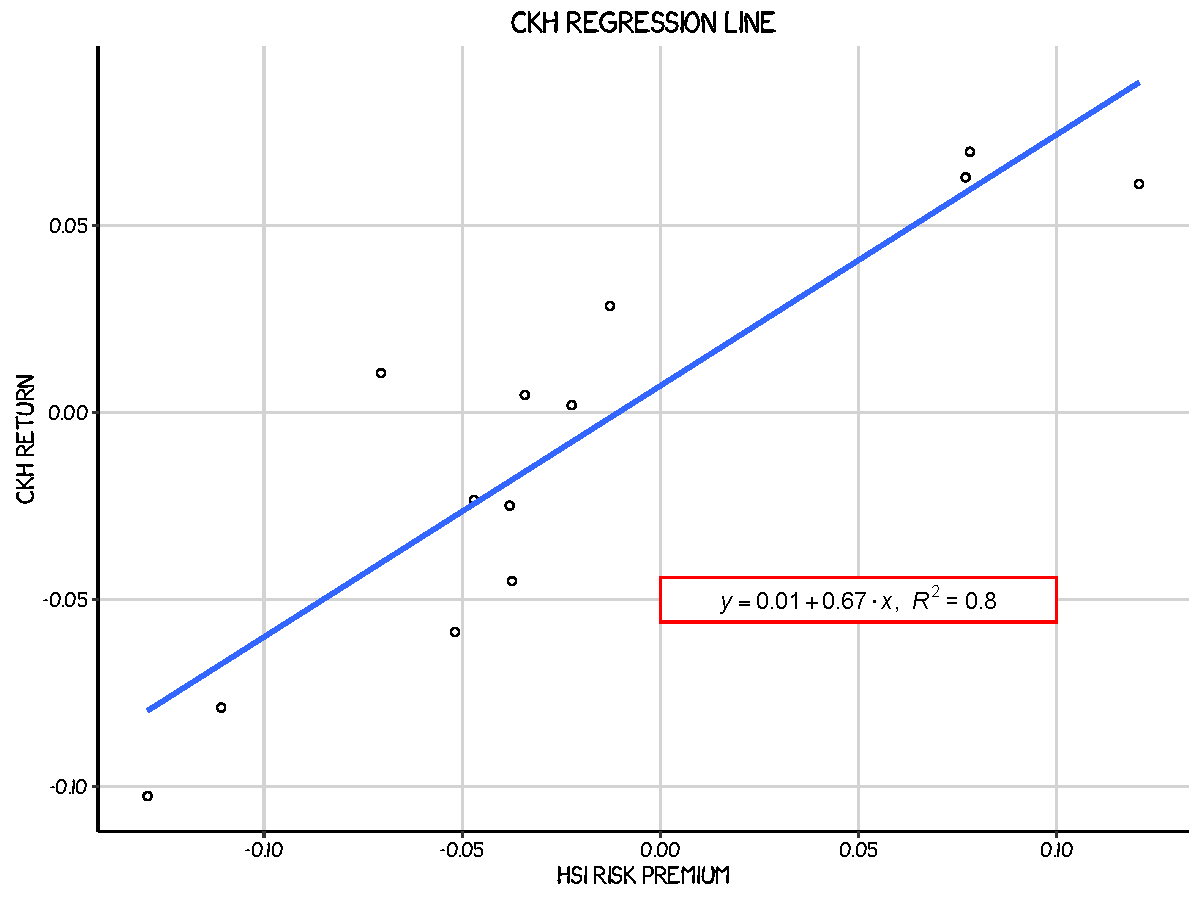
\includegraphics[width=0.55\linewidth]{figures/lr_15-1} \end{center}

\subsection{\texorpdfstring{Using `The Economist'
theme}{Using The Economist theme}}\label{using-the-economist-theme-10}

There are a wider range of pre-built themes available as part of the
\texttt{ggthemes} package (more information on these
\href{https://cran.r-project.org/web/packages/ggthemes/vignettes/ggthemes.html}{here}).
Below we've applied \texttt{theme\_economist()}, which approximates
graphs in the Economist magazine.

\begin{Shaded}
\begin{Highlighting}[]
\KeywordTok{library}\NormalTok{(ggthemes)}
\KeywordTok{library}\NormalTok{(grid)}

\NormalTok{fill <-}\StringTok{ "#4271AE"}
\NormalTok{line <-}\StringTok{ "#1F3552"}

\NormalTok{p11 <-}\StringTok{ }\KeywordTok{ggplot}\NormalTok{(hsi.ckh.returns, }\KeywordTok{aes}\NormalTok{(}\DataTypeTok{x=}\NormalTok{hsi.Risk.premium, }\DataTypeTok{y=}\NormalTok{ckh.Return)) +}
\StringTok{       }\KeywordTok{geom_point}\NormalTok{(}\DataTypeTok{shape=}\DecValTok{1}\NormalTok{) +}\StringTok{ }\KeywordTok{geom_smooth}\NormalTok{(}\DataTypeTok{method=}\NormalTok{lm, }\DataTypeTok{se=}\OtherTok{FALSE}\NormalTok{) +}
\StringTok{       }\KeywordTok{ggtitle}\NormalTok{(}\StringTok{"CKH regression line"}\NormalTok{) +}
\StringTok{       }\KeywordTok{scale_x_continuous}\NormalTok{(}\DataTypeTok{name =} \StringTok{"HSI risk premium"}\NormalTok{) +}
\StringTok{       }\KeywordTok{scale_y_continuous}\NormalTok{(}\DataTypeTok{name =} \StringTok{"CKH return"}\NormalTok{) +}
\StringTok{       }\KeywordTok{annotate}\NormalTok{(}\StringTok{"rect"}\NormalTok{, }\DataTypeTok{xmin =} \FloatTok{-0.002}\NormalTok{, }\DataTypeTok{xmax =} \FloatTok{0.102}\NormalTok{, }\DataTypeTok{ymin =} \NormalTok{-}\FloatTok{0.056}\NormalTok{, }
\StringTok{        }\DataTypeTok{ymax =} \NormalTok{-}\FloatTok{0.044}\NormalTok{, }\DataTypeTok{fill=}\StringTok{"white"}\NormalTok{, }\DataTypeTok{colour=}\StringTok{"red"}\NormalTok{) +}\StringTok{ }
\StringTok{       }\KeywordTok{annotate}\NormalTok{(}\StringTok{"text"}\NormalTok{, }\DataTypeTok{x =} \FloatTok{0.05}\NormalTok{, }\DataTypeTok{y =} \NormalTok{-}\FloatTok{0.05}\NormalTok{, }\DataTypeTok{label =} \KeywordTok{equation}\NormalTok{(fit), }
\StringTok{        }\DataTypeTok{parse =} \OtherTok{TRUE}\NormalTok{) +}\StringTok{ }
\StringTok{       }\KeywordTok{theme_economist}\NormalTok{() +}
\StringTok{       }\KeywordTok{theme}\NormalTok{(}\DataTypeTok{axis.line.x =} \KeywordTok{element_line}\NormalTok{(}\DataTypeTok{size=}\NormalTok{.}\DecValTok{5}\NormalTok{, }\DataTypeTok{colour =} \StringTok{"black"}\NormalTok{),}
\StringTok{        }\DataTypeTok{axis.line.y =} \KeywordTok{element_line}\NormalTok{(}\DataTypeTok{size=}\NormalTok{.}\DecValTok{5}\NormalTok{, }\DataTypeTok{colour =} \StringTok{"black"}\NormalTok{), }
\StringTok{        }\DataTypeTok{axis.text.x=}\KeywordTok{element_text}\NormalTok{(}\DataTypeTok{colour=}\StringTok{"black"}\NormalTok{, }\DataTypeTok{size =} \DecValTok{9}\NormalTok{), }
\StringTok{        }\DataTypeTok{axis.text.y=}\KeywordTok{element_text}\NormalTok{(}\DataTypeTok{colour=}\StringTok{"black"}\NormalTok{, }\DataTypeTok{size =} \DecValTok{9}\NormalTok{),}
\StringTok{        }\DataTypeTok{panel.grid.major =} \KeywordTok{element_line}\NormalTok{(}\DataTypeTok{colour =} \StringTok{"#d3d3d3"}\NormalTok{), }
\StringTok{        }\DataTypeTok{panel.grid.minor =} \KeywordTok{element_blank}\NormalTok{(), }
\StringTok{        }\DataTypeTok{panel.border =} \KeywordTok{element_blank}\NormalTok{(), }\DataTypeTok{panel.background =} \KeywordTok{element_blank}\NormalTok{(),}
\StringTok{        }\DataTypeTok{plot.title =} \KeywordTok{element_text}\NormalTok{(}\DataTypeTok{family =} \StringTok{"OfficinaSanITC-Book"}\NormalTok{),}
\StringTok{        }\DataTypeTok{text=}\KeywordTok{element_text}\NormalTok{(}\DataTypeTok{family=}\StringTok{"OfficinaSanITC-Book"}\NormalTok{))}
\NormalTok{p11}
\end{Highlighting}
\end{Shaded}

\begin{center}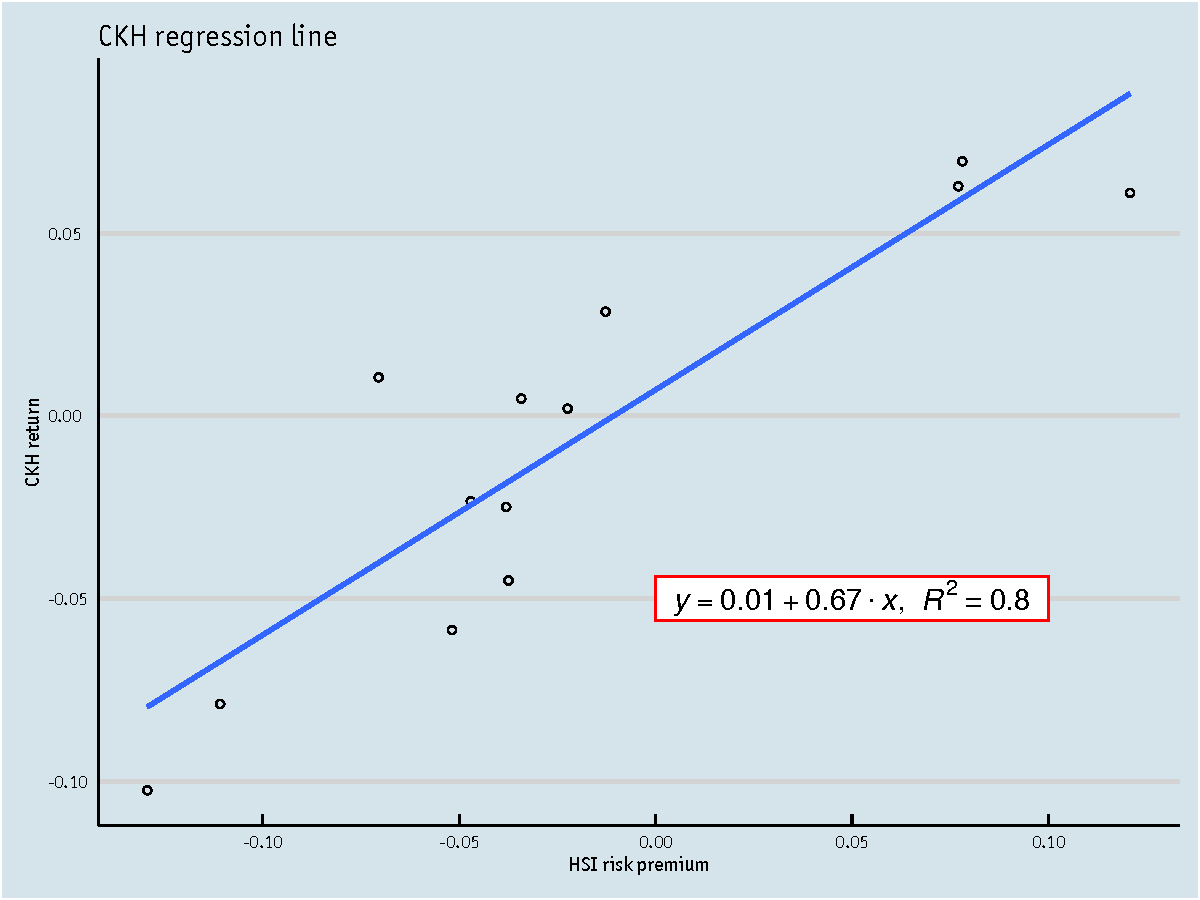
\includegraphics[width=0.55\linewidth]{figures/lr_16-1} \end{center}

\subsection{Creating your own
theme}\label{creating-your-own-theme-10}

As before, you can modify your plots a lot as \texttt{ggplot2} allows
many customisations. Here is a custom plot where we have modified the
axes, background and font.

\begin{Shaded}
\begin{Highlighting}[]
\KeywordTok{library}\NormalTok{(grid) }

\NormalTok{fill <-}\StringTok{ "#4271AE"}
\NormalTok{lines <-}\StringTok{ "#1F3552"}

\NormalTok{p11 <-}\StringTok{ }\KeywordTok{ggplot}\NormalTok{(hsi.ckh.returns, }\KeywordTok{aes}\NormalTok{(}\DataTypeTok{x=}\NormalTok{hsi.Risk.premium, }\DataTypeTok{y=}\NormalTok{ckh.Return)) +}
\StringTok{       }\KeywordTok{geom_point}\NormalTok{(}\DataTypeTok{shape=}\DecValTok{1}\NormalTok{) +}\StringTok{ }\KeywordTok{geom_smooth}\NormalTok{(}\DataTypeTok{method=}\NormalTok{lm, }\DataTypeTok{se=}\OtherTok{FALSE}\NormalTok{) +}
\StringTok{       }\KeywordTok{ggtitle}\NormalTok{(}\StringTok{"CKH regression line"}\NormalTok{) +}
\StringTok{       }\KeywordTok{scale_x_continuous}\NormalTok{(}\DataTypeTok{name =} \StringTok{"HSI risk premium"}\NormalTok{) +}
\StringTok{       }\KeywordTok{scale_y_continuous}\NormalTok{(}\DataTypeTok{name =} \StringTok{"CKH return"}\NormalTok{) +}
\StringTok{       }\KeywordTok{annotate}\NormalTok{(}\StringTok{"rect"}\NormalTok{, }\DataTypeTok{xmin =} \FloatTok{0.00}\NormalTok{, }\DataTypeTok{xmax =} \FloatTok{0.1}\NormalTok{, }\DataTypeTok{ymin =} \NormalTok{-}\FloatTok{0.056}\NormalTok{, }\DataTypeTok{ymax =} \NormalTok{-}\FloatTok{0.044}\NormalTok{, }
\StringTok{        }\DataTypeTok{fill=}\StringTok{"white"}\NormalTok{, }\DataTypeTok{colour=}\StringTok{"red"}\NormalTok{) +}\StringTok{ }
\StringTok{       }\KeywordTok{annotate}\NormalTok{(}\StringTok{"text"}\NormalTok{, }\DataTypeTok{x =} \FloatTok{0.05}\NormalTok{, }\DataTypeTok{y =} \NormalTok{-}\FloatTok{0.05}\NormalTok{, }\DataTypeTok{label =} \KeywordTok{equation}\NormalTok{(fit), }\DataTypeTok{parse =} \OtherTok{TRUE}\NormalTok{) +}\StringTok{ }
\StringTok{       }\KeywordTok{theme}\NormalTok{(}\DataTypeTok{axis.line.x =} \KeywordTok{element_line}\NormalTok{(}\DataTypeTok{size=}\NormalTok{.}\DecValTok{5}\NormalTok{, }\DataTypeTok{colour =} \StringTok{"black"}\NormalTok{),}
\StringTok{        }\DataTypeTok{axis.line.y =} \KeywordTok{element_line}\NormalTok{(}\DataTypeTok{size=}\NormalTok{.}\DecValTok{5}\NormalTok{, }\DataTypeTok{colour =} \StringTok{"black"}\NormalTok{),}
\StringTok{        }\DataTypeTok{axis.text.x=}\KeywordTok{element_text}\NormalTok{(}\DataTypeTok{colour=}\StringTok{"black"}\NormalTok{, }\DataTypeTok{size =} \DecValTok{9}\NormalTok{), }
\StringTok{        }\DataTypeTok{axis.text.y=}\KeywordTok{element_text}\NormalTok{(}\DataTypeTok{colour=}\StringTok{"black"}\NormalTok{, }\DataTypeTok{size =} \DecValTok{9}\NormalTok{), }
\StringTok{        }\DataTypeTok{legend.position =} \StringTok{"bottom"}\NormalTok{, }\DataTypeTok{legend.position =} \StringTok{"horizontal"}\NormalTok{,}
\StringTok{        }\DataTypeTok{panel.grid.major =} \KeywordTok{element_line}\NormalTok{(}\DataTypeTok{colour =} \StringTok{"#d3d3d3"}\NormalTok{), }
\StringTok{        }\DataTypeTok{panel.grid.minor =} \KeywordTok{element_blank}\NormalTok{(), }
\StringTok{        }\DataTypeTok{panel.border =} \KeywordTok{element_blank}\NormalTok{(), }\DataTypeTok{panel.background =} \KeywordTok{element_blank}\NormalTok{(),}
\StringTok{        }\DataTypeTok{plot.title =} \KeywordTok{element_text}\NormalTok{(}\DataTypeTok{size =} \DecValTok{14}\NormalTok{, }\DataTypeTok{family =} \StringTok{"Tahoma"}\NormalTok{, }\DataTypeTok{face =} \StringTok{"bold"}\NormalTok{),}
\StringTok{        }\DataTypeTok{text=}\KeywordTok{element_text}\NormalTok{(}\DataTypeTok{family=}\StringTok{"Tahoma"}\NormalTok{))}
\NormalTok{p11}
\end{Highlighting}
\end{Shaded}

\begin{center}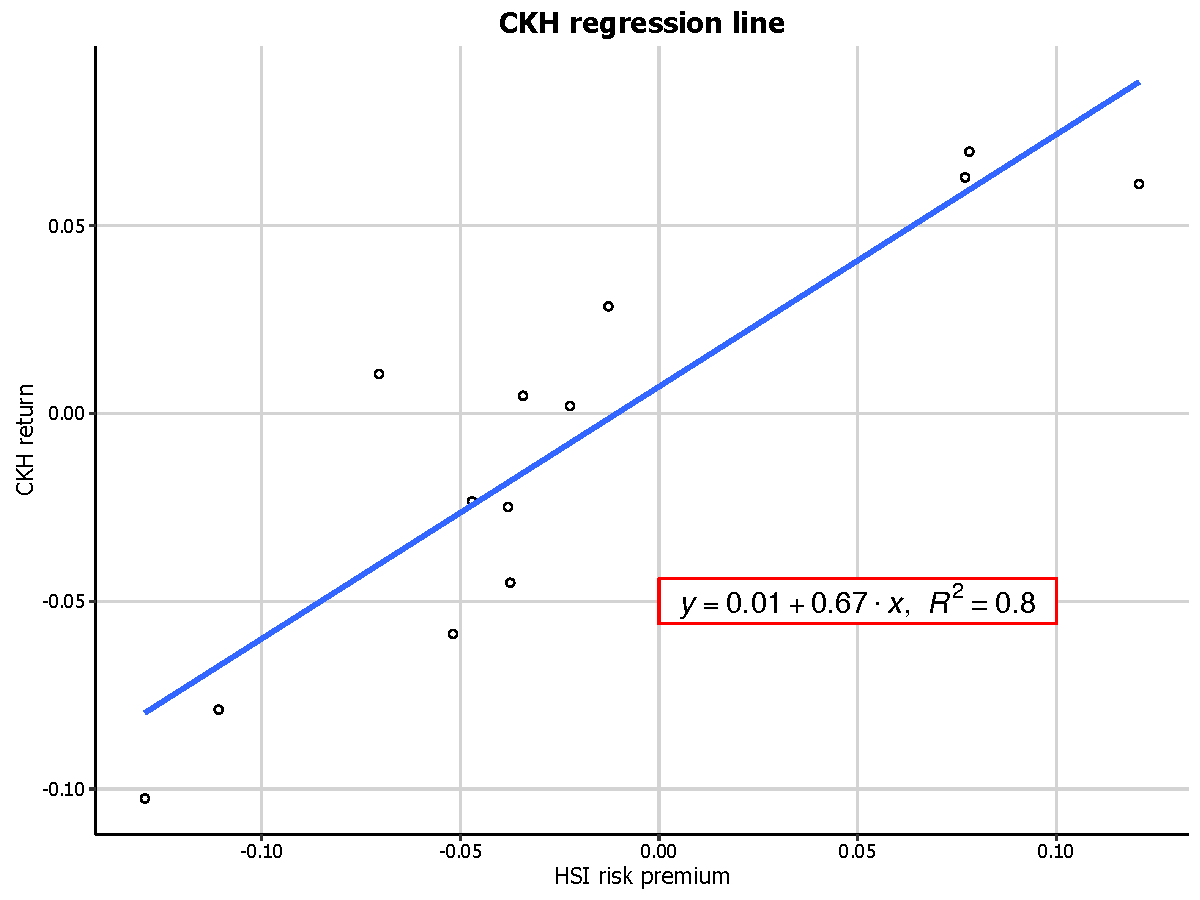
\includegraphics[width=0.55\linewidth]{figures/lr_17-1} \end{center}

\section{Regression diagnostics
plots}\label{regression-diagnostics-plots}

\subsection{Basic diagnostics plots}\label{basic-diagnostics-plots}

\texttt{ggfortify} lets \texttt{ggplot2} know how to interpret
\texttt{lm} objects.

\begin{Shaded}
\begin{Highlighting}[]
\CommentTok{# install.packages("ggfortify")}
\KeywordTok{library}\NormalTok{(ggfortify)}
\KeywordTok{autoplot}\NormalTok{(fit, }\DataTypeTok{label.size =} \DecValTok{3}\NormalTok{)}
\end{Highlighting}
\end{Shaded}

\begin{center}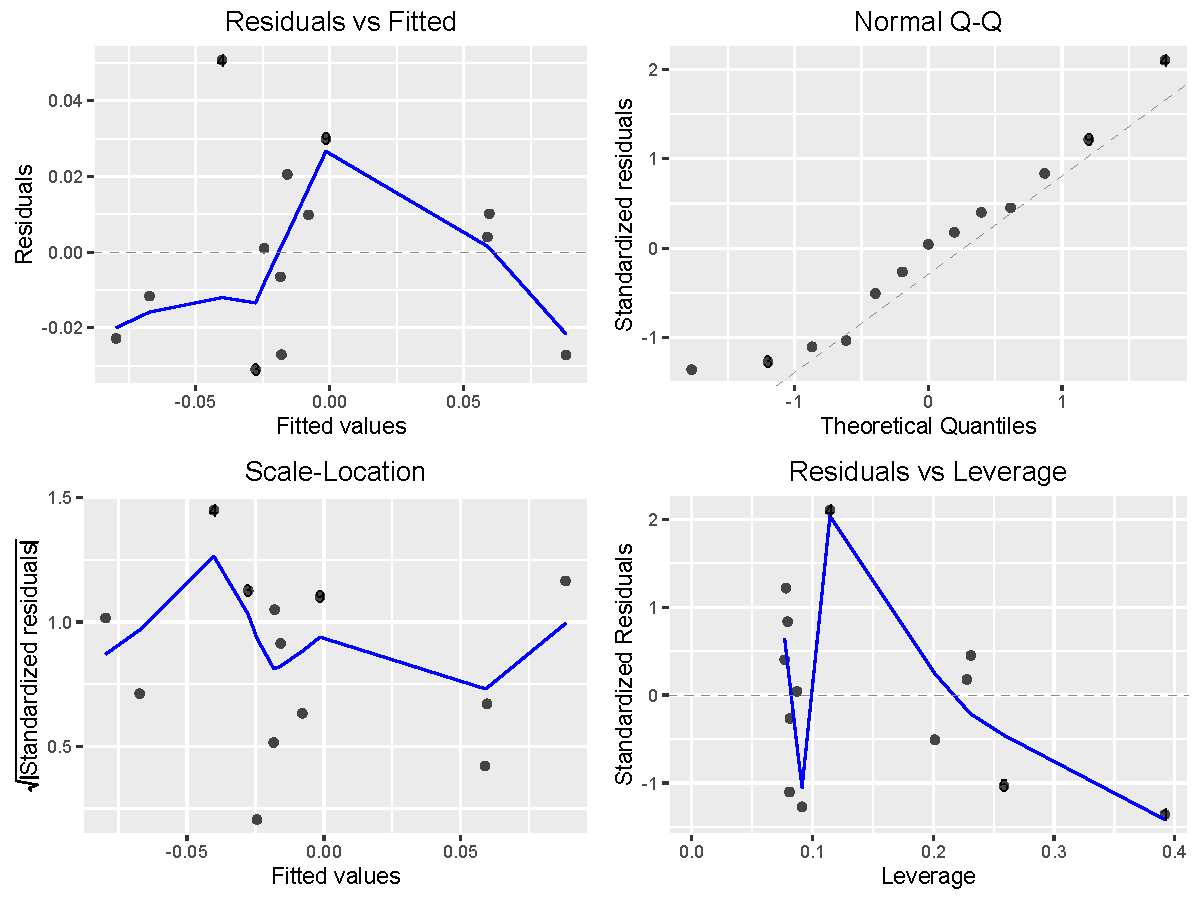
\includegraphics[width=0.55\linewidth]{figures/lr_18-1} \end{center}

\subsection{Using the white theme}\label{using-the-white-theme-11}

\begin{Shaded}
\begin{Highlighting}[]
\KeywordTok{autoplot}\NormalTok{(fit, }\DataTypeTok{label.size =} \DecValTok{3}\NormalTok{) +}\StringTok{ }\KeywordTok{theme_bw}\NormalTok{()}
\end{Highlighting}
\end{Shaded}

\begin{center}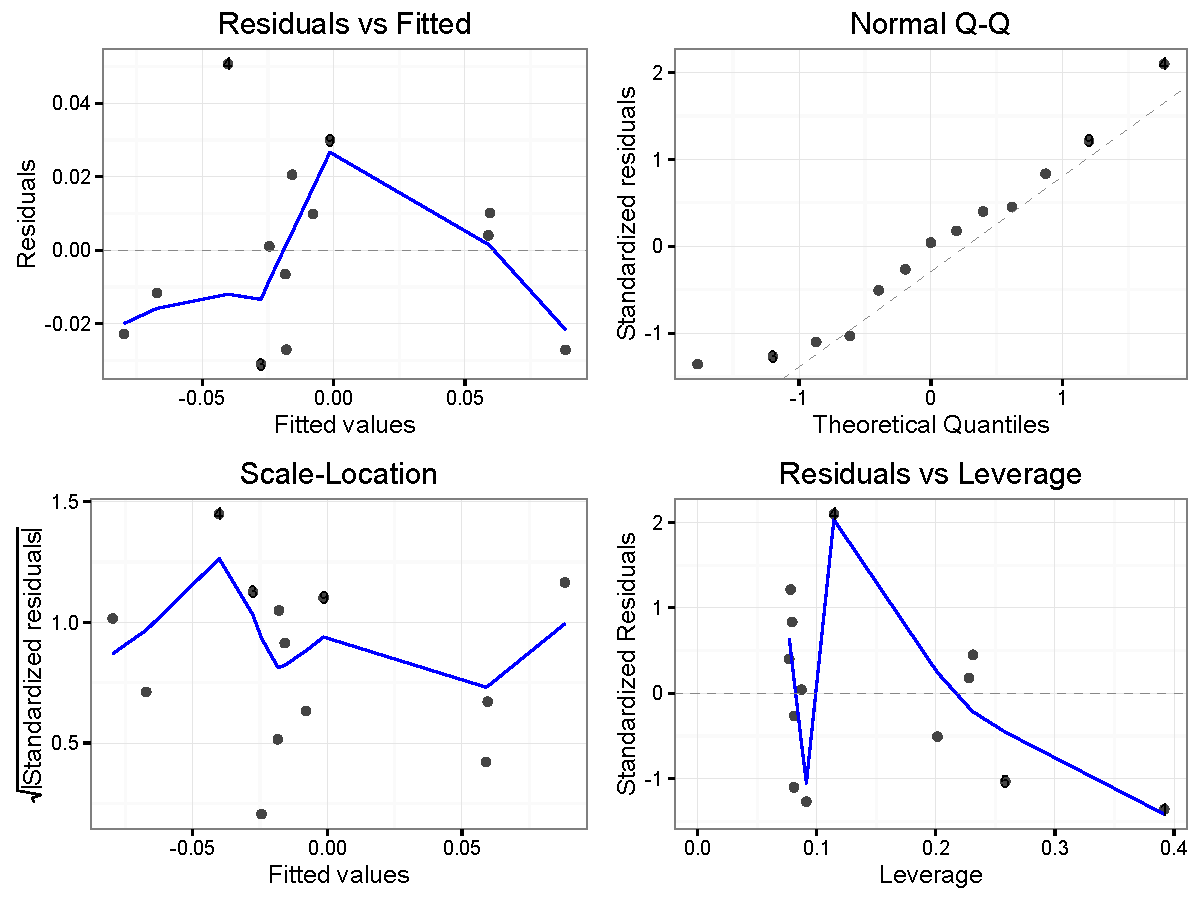
\includegraphics[width=0.55\linewidth]{figures/lr_19-1} \end{center}

\subsection{Creating an XKCD style
chart}\label{creating-an-xkcd-style-chart-11}

\begin{Shaded}
\begin{Highlighting}[]
\KeywordTok{autoplot}\NormalTok{(fit, }\DataTypeTok{label.size =} \DecValTok{3}\NormalTok{) +}\StringTok{ }\KeywordTok{theme}\NormalTok{(}\DataTypeTok{axis.line.x =} \KeywordTok{element_line}\NormalTok{(}\DataTypeTok{size=}\NormalTok{.}\DecValTok{5}\NormalTok{, }
\StringTok{        }\DataTypeTok{colour =} \StringTok{"black"}\NormalTok{),}
\StringTok{        }\DataTypeTok{axis.line.y =} \KeywordTok{element_line}\NormalTok{(}\DataTypeTok{size=}\NormalTok{.}\DecValTok{5}\NormalTok{, }\DataTypeTok{colour =} \StringTok{"black"}\NormalTok{), }
\StringTok{        }\DataTypeTok{axis.text.x=}\KeywordTok{element_text}\NormalTok{(}\DataTypeTok{colour=}\StringTok{"black"}\NormalTok{, }\DataTypeTok{size =} \DecValTok{9}\NormalTok{), }
\StringTok{        }\DataTypeTok{axis.text.y=}\KeywordTok{element_text}\NormalTok{(}\DataTypeTok{colour=}\StringTok{"black"}\NormalTok{, }\DataTypeTok{size =} \DecValTok{9}\NormalTok{),}
\StringTok{        }\DataTypeTok{panel.grid.major =} \KeywordTok{element_line}\NormalTok{(}\DataTypeTok{colour =} \StringTok{"#d3d3d3"}\NormalTok{), }
\StringTok{        }\DataTypeTok{panel.grid.minor =} \KeywordTok{element_blank}\NormalTok{(), }
\StringTok{        }\DataTypeTok{panel.border =} \KeywordTok{element_blank}\NormalTok{(), }\DataTypeTok{panel.background =} \KeywordTok{element_blank}\NormalTok{(),}
\StringTok{        }\DataTypeTok{plot.title =} \KeywordTok{element_text}\NormalTok{(}\DataTypeTok{family =} \StringTok{"xkcd-Regular"}\NormalTok{),}
\StringTok{        }\DataTypeTok{text=}\KeywordTok{element_text}\NormalTok{(}\DataTypeTok{family=}\StringTok{"xkcd-Regular"}\NormalTok{))}
\end{Highlighting}
\end{Shaded}

\begin{center}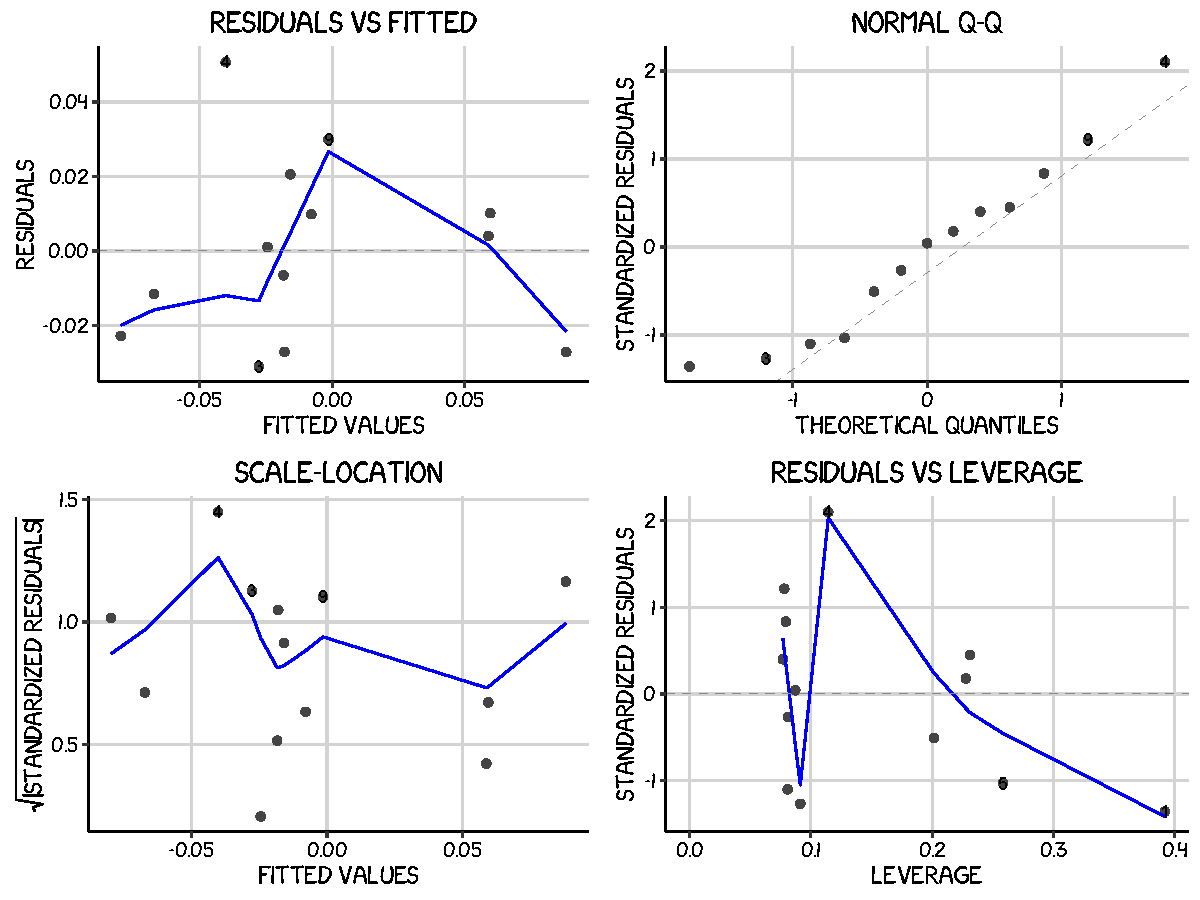
\includegraphics[width=0.55\linewidth]{figures/lr_20-1} \end{center}

\subsection{\texorpdfstring{Using `The Economist'
theme}{Using The Economist theme}}\label{using-the-economist-theme-11}

\begin{Shaded}
\begin{Highlighting}[]
\KeywordTok{autoplot}\NormalTok{(fit, }\DataTypeTok{label.size =} \DecValTok{3}\NormalTok{) +}\StringTok{ }\KeywordTok{theme_economist}\NormalTok{() +}
\StringTok{        }\KeywordTok{theme}\NormalTok{(}\DataTypeTok{axis.line.x =} \KeywordTok{element_line}\NormalTok{(}\DataTypeTok{size=}\NormalTok{.}\DecValTok{5}\NormalTok{, }\DataTypeTok{colour =} \StringTok{"black"}\NormalTok{),}
\StringTok{         }\DataTypeTok{axis.line.y =} \KeywordTok{element_line}\NormalTok{(}\DataTypeTok{size=}\NormalTok{.}\DecValTok{5}\NormalTok{, }\DataTypeTok{colour =} \StringTok{"black"}\NormalTok{), }
\StringTok{         }\DataTypeTok{axis.text.x=}\KeywordTok{element_text}\NormalTok{(}\DataTypeTok{colour=}\StringTok{"black"}\NormalTok{, }\DataTypeTok{size =} \DecValTok{9}\NormalTok{), }
\StringTok{         }\DataTypeTok{axis.text.y=}\KeywordTok{element_text}\NormalTok{(}\DataTypeTok{colour=}\StringTok{"black"}\NormalTok{, }\DataTypeTok{size =} \DecValTok{9}\NormalTok{),}
\StringTok{         }\DataTypeTok{panel.grid.major =} \KeywordTok{element_line}\NormalTok{(}\DataTypeTok{colour =} \StringTok{"#d3d3d3"}\NormalTok{), }
\StringTok{         }\DataTypeTok{panel.grid.minor =} \KeywordTok{element_blank}\NormalTok{(), }
\StringTok{         }\DataTypeTok{panel.border =} \KeywordTok{element_blank}\NormalTok{(), }\DataTypeTok{panel.background =} \KeywordTok{element_blank}\NormalTok{(),}
\StringTok{         }\DataTypeTok{plot.title =} \KeywordTok{element_text}\NormalTok{(}\DataTypeTok{family =} \StringTok{"OfficinaSanITC-Book"}\NormalTok{),}
\StringTok{         }\DataTypeTok{text=}\KeywordTok{element_text}\NormalTok{(}\DataTypeTok{family=}\StringTok{"OfficinaSanITC-Book"}\NormalTok{))}
\end{Highlighting}
\end{Shaded}

\begin{center}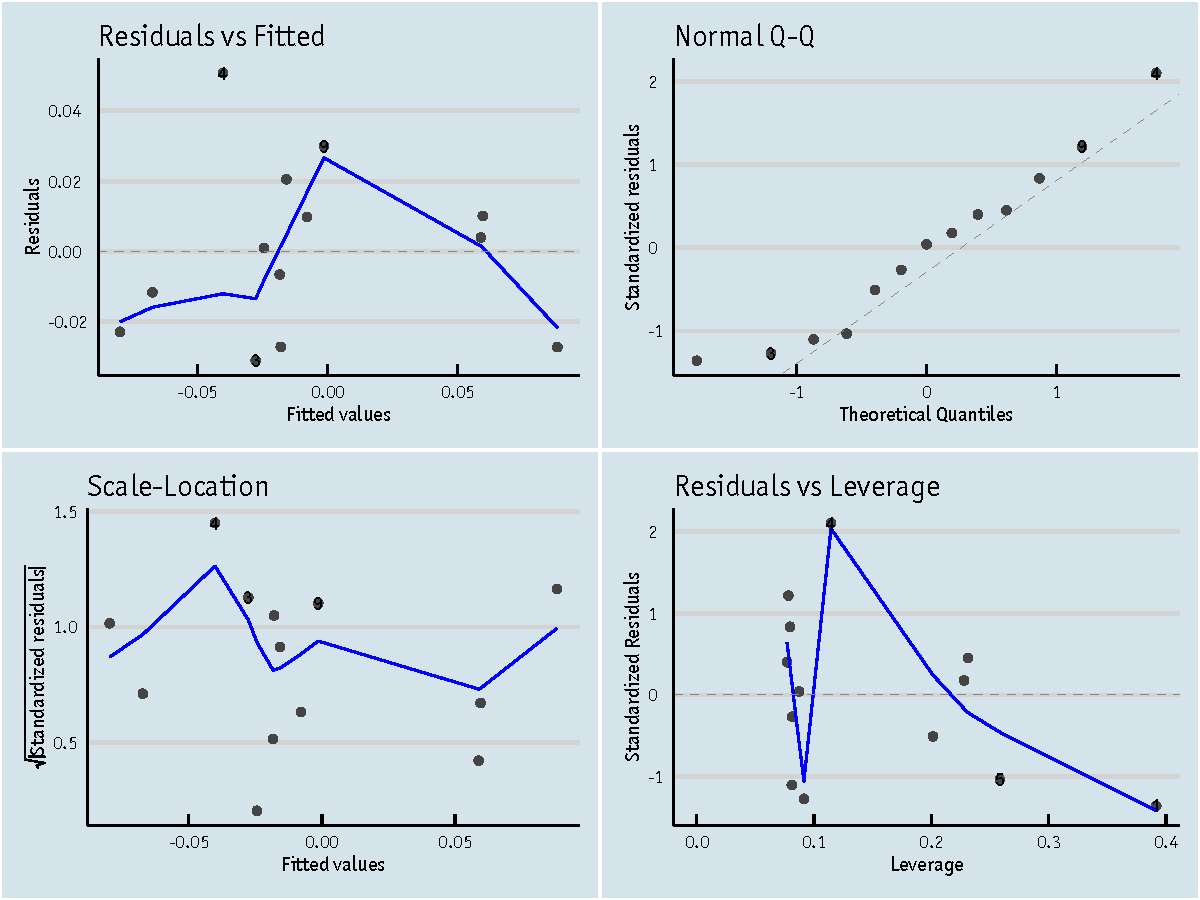
\includegraphics[width=0.55\linewidth]{figures/lr_21-1} \end{center}

\subsection{Creating your own
theme}\label{creating-your-own-theme-11}

\begin{Shaded}
\begin{Highlighting}[]
\KeywordTok{autoplot}\NormalTok{(fit, }\DataTypeTok{label.size =} \DecValTok{3}\NormalTok{) +}\StringTok{ }\KeywordTok{theme}\NormalTok{(}\DataTypeTok{axis.line.x =} \KeywordTok{element_line}\NormalTok{(}\DataTypeTok{size=}\NormalTok{.}\DecValTok{5}\NormalTok{, }
\StringTok{        }\DataTypeTok{colour =} \StringTok{"black"}\NormalTok{),}
\StringTok{        }\DataTypeTok{axis.line.y =} \KeywordTok{element_line}\NormalTok{(}\DataTypeTok{size=}\NormalTok{.}\DecValTok{5}\NormalTok{, }\DataTypeTok{colour =} \StringTok{"black"}\NormalTok{),}
\StringTok{        }\DataTypeTok{axis.text.x=}\KeywordTok{element_text}\NormalTok{(}\DataTypeTok{colour=}\StringTok{"black"}\NormalTok{, }\DataTypeTok{size =} \DecValTok{9}\NormalTok{), }
\StringTok{        }\DataTypeTok{axis.text.y=}\KeywordTok{element_text}\NormalTok{(}\DataTypeTok{colour=}\StringTok{"black"}\NormalTok{, }\DataTypeTok{size =} \DecValTok{9}\NormalTok{), }
\StringTok{        }\DataTypeTok{legend.position =} \StringTok{"bottom"}\NormalTok{, }\DataTypeTok{legend.position =} \StringTok{"horizontal"}\NormalTok{,}
\StringTok{        }\DataTypeTok{panel.grid.major =} \KeywordTok{element_line}\NormalTok{(}\DataTypeTok{colour =} \StringTok{"#d3d3d3"}\NormalTok{), }
\StringTok{        }\DataTypeTok{panel.grid.minor =} \KeywordTok{element_blank}\NormalTok{(), }
\StringTok{        }\DataTypeTok{panel.border =} \KeywordTok{element_blank}\NormalTok{(), }\DataTypeTok{panel.background =} \KeywordTok{element_blank}\NormalTok{(),}
\StringTok{        }\DataTypeTok{plot.title =} \KeywordTok{element_text}\NormalTok{(}\DataTypeTok{size =} \DecValTok{14}\NormalTok{, }\DataTypeTok{family =} \StringTok{"Tahoma"}\NormalTok{, }\DataTypeTok{face =} \StringTok{"bold"}\NormalTok{),}
\StringTok{        }\DataTypeTok{text=}\KeywordTok{element_text}\NormalTok{(}\DataTypeTok{family=}\StringTok{"Tahoma"}\NormalTok{))}
\end{Highlighting}
\end{Shaded}

\begin{center}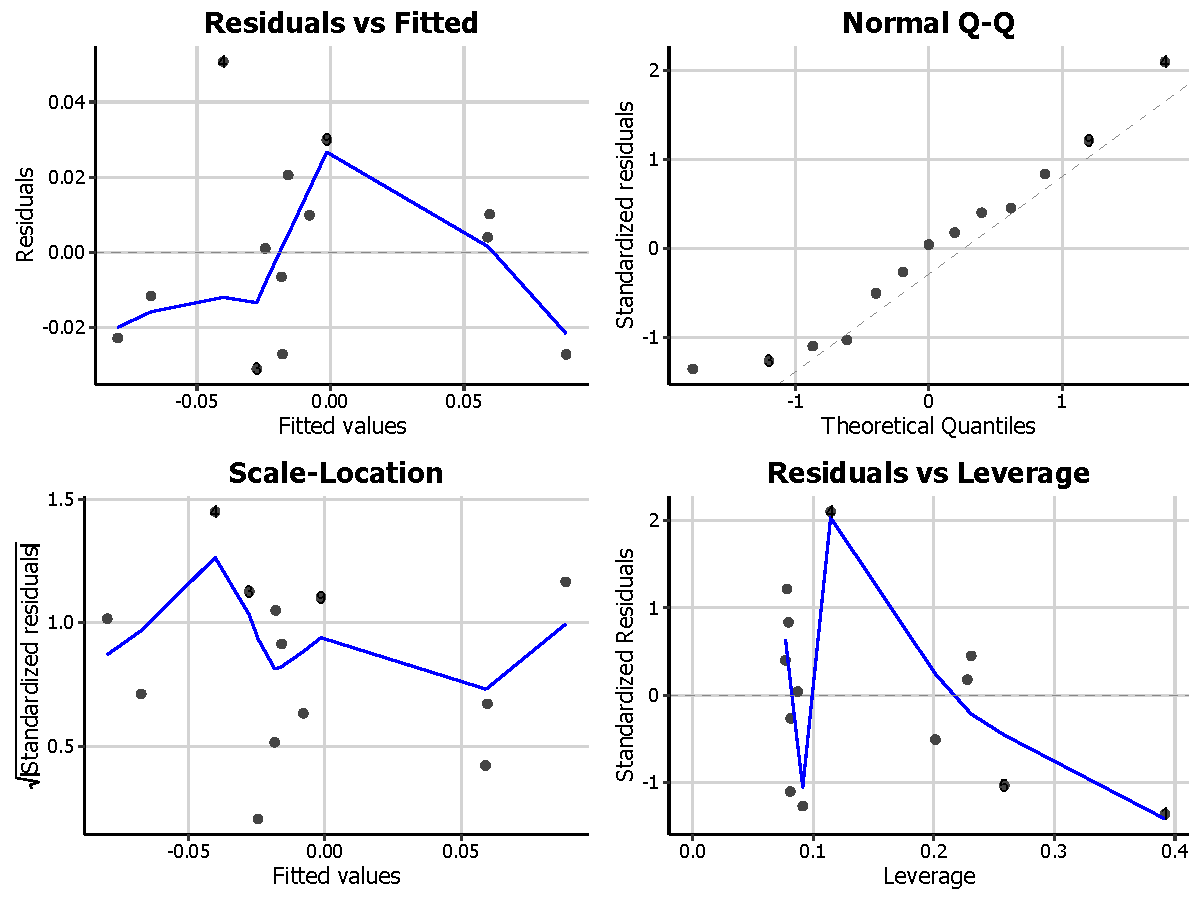
\includegraphics[width=0.55\linewidth]{figures/lr_22-1} \end{center}